\title{Crowdsourced Residential Power Quality Event Detection in the Smart Grid.}
\author{
        Sergey Negrashov \\
                Department of Information and Computer Science\\
}
\date{\today}

\documentclass[11pt]{uhthesis}
\author{Sergey Negrashov}
%% Month in which you intend to receive your degree (i.e. graduation).
%% Presumably this will be one of: May, August, or December.
\degreemonth{December}
%% Year of expected graduation.
\degreeyear{2019}
%% Type of degree to be conferred.
\degree{Doctor of Philosophy}
%% This is the chairperson of your committee. Do not use titles like Dr.
\chair{Philip Johnson}
%% The other members of your committee, seperated by "\\". Again, no titles,
%% and it is customary to list the outside committee member (if you have one)
%% last.
\othermembers{Peter-Michael Seidel\\
Edo Biagioni\\
Lipyeow Lim
}
%% The field in which you are obtaining your degree, capitalized normally.
\field{Computer Science}
%% If your discipline allows subfields, you can add it here. Note that this
%% is strictly controlled, so consult the Style & Policy guide before adding
%% a subfield.
%\subfield{Bioinformatics}
%% 4-6 optional keywords/phrases for use in indexing or as search terms
\keywords{Sensor Network, Distributed Sensing, Grid Computing, Power Quality}
%% The version number of your document. Consistent use of this will enable you
%% to tell old drafts from new ones. Final actual documents omit this
%% automatically so you can use it without fear of submission problems at the
%% end. If you do not define this parameter, it defaults to "1.0.0".
\versionnum{4.0.0}

%%% End of preamble

\usepackage{graphicx}
\usepackage{wrapfig}

\usepackage{indentfirst}
\usepackage{caption}
\usepackage{subcaption}

\begin{document}
\maketitle

\begin{frontmatter}

%%% Note, there is no longer a signature page included in the document, it
%%% has been replaced by Form IV

%%% Create the copyright page (optional)
\copyrightpage

%%% Bring in the dedication page from external file (optional)
\include{dedication}

%%% Bring in the acknowledgments section from external file (optional)
\include{acknowledgments}

%%% Bring in the abstract section from external file
\begin{abstract}
Today`s big data world, is heavily relied on to bring precise, timely, and actionable intelligence, while being burdened by the ever increasing need for data cleaning and preprocessing. While in the case of ingesting large quantity of unstructured data this problem is unavoidable, when it comes to sensor networks built for a specific purpose, such as anomaly detection, some of that computation can be moved to the edge of the network. This thesis concerns the special case of sensor networks tailored for monitoring the power grid for anomalous behavior. These networks consist of meters connected to the grid across multiple geographically separated locations, while monitoring the power delivery infrastructure with the intent of finding deviations from the nominal steady state. These deviations, known as power quality anomalies, may originate, and be localized to the location the sensor is located, or may affect a sizable portion of the power grid. The difficulty of evaluating the extent of the power quality anomaly stems directly from their short temporal and variable geographical impact. I propose a novel distributed power quality monitoring system called Napali which relies on extracted metrics from individual meters and their temporal locality in order to intelligently detect anomalies and extract raw data within temporal window and geographical areas of interest. The results of this research should be useful in other disciplines, such as general sensor network applications, IOT, and intrusion detection systems.
\end{abstract}


%%% Generate table of contents
\tableofcontents

%%% Generate list of tables
\listoftables

%%% Generate list of figures
\listoffigures

\end{frontmatter}

\chapter{Introduction}

Power quality research is a subset of power distribution research which focuses on studying  deviations from nominal power grid operating conditions. Devices connected to the power grid, as well as the distribution equipment expect a certain frequency, voltage and harmonic content of the voltage waveform they operate on. While most equipment maintains some hysteresis with respect to deviations from the nominal, large enough deviations may cause equipment failure and instability in the power grid as a whole. In a practical sense, power quality monitoring concerns itself with monitoring, collecting and analyzing power quality anomalies on a live and functioning grid. In some cases, for example when performed by the utility, this information is used to make real-time decisions, to maintain the stability of the power grid. However, data collected by the power quality monitoring equipment can also be used to diagnose local power quality problems, or to further power quality research. Power quality monitoring fits very well into the paradigm of remote sensing and sensor networks, particularly into the newly emerging field of edge computing. Edge computing goes beyond the naive approach of transmitting the entirety of the collected data from the sensor location, and extends it by either feature extracting, preprocessing or filtering the data at the computing node itself. This research project will investigate the design, implementation, and evaluation of a novel edge computing architecture called Napali which combines feature extraction at the edge level and two way communication between the sink and the edge node. I will evaluate Napali in part by implementing it in the power quality monitoring domain.

\section{Overview of power grids}
Modern power grids are hierarchically structured. Higher voltage is useful for transporting electricity over long distances, connecting cities and towns to power generation facilities. Transmissions lines of 100kV and above are used to minimize losses in long distance runs, since the same amount of power can be transmitted using much lower current, and thus much more efficiently, then the comparable low voltage line. Close to the point of distribution, transmission voltage is stepped down to 1kV-40kV range using large power transformers. This is done because the losses incurred in the final leg of transmission are minimal, while extremely high voltage equipment is expensive and requires special precautions.\cite{sivanagaraju2008electric} Finally, at the consumer level the voltage level is stepped down once more to the household voltage, for example $120V_{ac}$ for North America. It is important to note that voltage across every part of the power grid is synchronized to a phase and frequency set by the utility. This allows multiple power producers to contribute to electricity generation without interfering with each other.\cite{blaabjerg2006overview} In North America the 60Hz utility frequency is used as the baseline, and its long term stability is guaranteed by the power company. How close the power AC frequency is to the nominal value is a measure of how closely the electricity demand is balanced by the electricity generation. 

Traditional power generation sources involves applying mechanical torque to an alternating current generator. If the load on the generator increases without increasing the torque, it will slow down the generator and thus the utility frequency decreases. Similarly, if the demand drops but the torque is not decreased, the frequency of generated power will increase. Even small deviations in frequency can have adverse effects on equipment which runs synchronous to the power grid, such as synchronous electric motors and other industrial equipment.\cite{morren2006wind} Nonlinear loads, or loads that don't draw a consistent amount of current through out an AC cycle, are highly prevalent in today's power grid. These devices contribute to the harmonic noise in power system in both current and voltage waveform. This effect, known as harmonic distortion, can have various unintended consequences on the power distribution system and connected devices. The current harmonic distortion affects the efficiency of the distribution network, while voltage harmonics may propagate across the power distribution infrastructure and affect neighboring devices.\cite{muhamad2007effects} Distributed renewable generation may also create untended harmonics. Distributed generators are commonly DC systems, which utilize inverters to generate in phase AC waveform to feed into the power grid. Depending on the inverter design the AC waveform may have spurious harmonics present.\cite{morren2006wind} 

Large and sudden changes in load to generation ratio change do not immediately impact the utility frequency due to the rotational inertia of the large generation systems. Instead it will cause the line voltage to change proportional to the load until the generation can catch up. If the load suddenly increases, caused for example by a large motor stall, grid voltage will experience a sharp drop, known as a sag. Similarly a large load drop will cause an voltage increase, called a swell. Voltage sags and swells propagate throughout the entire grid infrastructure, however the dynamics of the power grid are quite complex, and hard to predict. For example a voltage sag on one sub-transmission chain may manifest and as a voltage swell in another. Finally very fast changes in load, such as short circuits, opening and closing of re-closers, and lightning strikes manifest as voltage transients. Voltage transients are energetic short-lived swells on the order of a single AC cycle, which can travel across the distribution grid. Transients may interfere with sensitive grid connected equipment, as well as trigger protection equipment such as uninterpretable power supplies, and other over-voltage protection devices. Transients, harmonic distortion, and RMS fluctuations and their combinations make up the majority of power quality problems which affect the voltage waveform in the grid connected devices. \cite{5154067} All of these issues can cause power quality problems, as will be discussed further in Section \ref{intro:sec:pq}.

\section{Edge computing approach to anomaly detection}\label{intro:edge}
Edge computing is an emergent field in distributed systems. Edge computing is a consequence of ever decreasing power consumption of computational devices found on the sensor nodes, as well as incremental improvements in battery technology. With ever-increasing computational capabilities in sensor networks, it becomes possible to process and store the acquired data on the device itself, as opposed to the centralized sink. Thus the idea of edge computing leverages available computing power of the sensor node to allow for smarter distributed sensing. Edge computing with respect to remote sensing allows for several new approaches to anomaly detection. 

Anomaly detection is a common topic across many disciplines and domains. In cyber-security research, anomalous network traffic and program behavior is often indicative of malicious behavior. In seismic monitoring, anomalies in ground vibrations may be precursors to an earthquake or a volcano eruption. In observational astronomy, anomaly detection is used for detection of transient events such as gamma ray bursts. Sensor networks are commonly tasked with anomaly detection and must often act on them. Traditionally, stringent constraints on power consumption of battery powered wireless sensor network nodes mean that low bandwidth and low complexity methods are preferred. Furthermore, many sensor networks are often hindered by local noise, thus requiring higher level filtering in order and in network processing to determine if an anomaly has occurred. If the signal to noise of the local measurements is quite high this problem becomes trivial: one simply collects all the distributed measurements if one or more of the measurements indicates an anomaly. Unfortunately, in the real world such problems are rare and instead the distributed signal is dominated by extraneous local noise. For example individual seismic sensors can't distinguish between a global anomaly such as an earthquake and local noise such as vibration caused by a passing semi-truck. 

The problem of global anomaly detection with distributed sensing has been thoroughly explored in self organizing wireless sensor networks. However, these approaches are insufficient in the paradigm of edge computing. Edge computing relies on Internet for transport, and thus the cost of communicating with the local sink and the local node is similar. Indeed in some cases it is impossible to achieve node-to-node communication without an intermediary due to firewalls, and other security mechanisms. In my research I will only consider approaches which rely on a sink node to facilitate anomaly detection.

There are several solutions for dealing with the local noise problem in an Internet-enabled sensor network. A naive solution is to simply record every distributed measurement to a centralized data sink. This sink, as well as the infrastructure down stream of it has a view of the entire state of the system and can thus detect anomalies using either real-time or batch processing. An alternative to sending all of the distributed measurements to the sink is to let the individual sensors decide which temporal regions of the measurement constitute an anomaly. This approach, called self triggering, has a benefit of the reducing the bandwidth constraints for each sensor without the requirement for two way communication between the sensor and the sink.

\section{Napali: hybrid edge computing for anomaly detection.} \label{intro:section:napali}
  
I propose a framework called Napali which combines the strengths of the previously mentioned methods. In Napali, each sensor node maintains a two way communication channel with the sink, as well as a temporal window containing all the recent data each device has collected. Each sensor's on board processing is used to extract features from the collected measurements, and only these features, instead of the entire measurement set are forwarded to the sink for processing. The sink has a low resolution view of the state of the entire sensor network. While this may not be enough for rigorous anomaly analysis, properly feature extracted data from every node should be enough to detect the occurrence of an anomaly. Finally if an anomaly is detected the sink will request high resolution data from all of the affected devices and their neighbors. 

\begin{figure}[h]
	  \centering
	  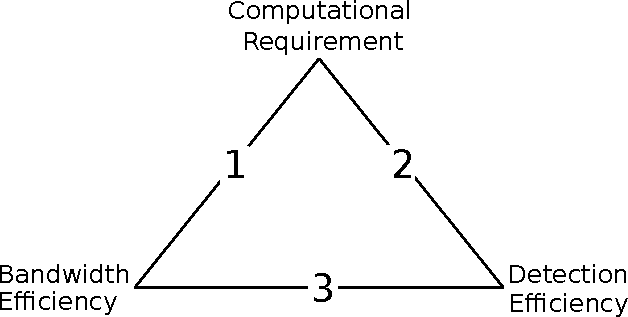
\includegraphics[width=0.5\linewidth]{img/edge_computing_vs.pdf}
	\caption{Comparison of the three event detection methodology across three metrics. Methods are as follows: naive method (2), self triggering (1), Napali, hybrid solution (3)}
	\label{intro:fig:edge}
\end{figure}
The naive method provides the best detection ability and the smallest node computation requirement. However, it does so at the cost of the largest bandwidth consumption. The self triggering method has the lowest bandwidth consumption of the three. The disadvantage of this method is twofold. First of all in order to maintain a high detection rate a reasonably low threshold for anomalies has to be used. This may cause a large number of false positives due to local noise and sensor noise. Secondly, global anomalies will often diminish in magnitude as a function of distance from the epicenter, thus far removed sensor nodes may completely miss events. These low threshold events may be invaluable for reconstructing the dynamic of the anomaly propagation, however they will be missed by the detection algorithms. 

Napali's hybrid approach provides the opportunity for much better anomaly detection rate and background noise rejection, by correlating the features that are computed on the sensor nodes. Napali has moderate bandwidth consumption, however the bandwidth consumption is tunable since the features can be computed for varied temporal windows length of which can be adjusted in real time. Napali does requires the highest sensor node computing power, since not only does it need to extract the triggering features from from raw data, it needs to maintain a buffer of sensor measurements to send to the sink if an anomaly is detected.

The downside of the Napali framework, is the requirement for two way communication between the sink and the sensor node. In order to participate in event detection Napali sensors need to be able to both send raw and feature extracted data, as well as receive the control signals from the sink. In contrast, the naive and self triggered approaches only require a one way link to send the raw data to the sink. As such, standalone devices can be retrofired to participate in distributed event detection in the naive and self triggered approaches, while Napali requires custom devices specifically tailored for cooperative event detection.

I claim that there are several benefits to the Napali method compared to the naive and self triggered approaches.
\begin{enumerate}
	\item \textbf{Bandwidth usage is minimized:} Instead of sending the entirety of raw data, only extracted features are sent. This features will have a tiny fraction of the bandwidth requirement when compared to raw waveforms. Furthermore, the temporal window which encompasses a single feature can be adjusted in real time. Thus as soon as an anomalous behavior is observed in a subset of sensors, this window can be adjusted for a finer grained feature extraction.
  
	\item \textbf{Effects of latency are minimized:} Even at 1Msample/second at 16bits of resolution, the memory requirement to store 5 minutes of raw waveform without compression are on the order of 512MB, which is well within the realm of cheap single board computers. With compression specifically suited to the signal of interest, the memory requirement can be reduced even further. This gives the triggering stream sink plenty of time to respond to the anomalies in the data and request raw waveform from the monitoring devices.
  
	\item \textbf{Sink processing requirements are minimized:} Since most of the feature extraction is already performed at the device level the triggering stream sink computational resources can be minimized. With the advent of IOT, the computational capacity of the edge devices is quickly growing. Napali exploits these resources, and thus minimizes the sink computational requirements.
  
	\item \textbf{Sub-threshold data acquisition:} The triggering stream sink makes the decision to acquire raw waveform from sensor nodes. This allows researchers to collect data from devices which were only mildly affected or not affected by the disturbance. This provides new possibilities for investigation of disturbance propagation across the sensed area.
  
	\item \textbf{Power failure resiliency:} In the case of the complete power failure or communication blackout, if the monitoring device has a battery backup capability, each sensor has a record of the entire raw waveform leading up to the power interruption. Prior to shutdown the sensor node will transfer all of the raw data from the volatile memory to on-board permanent storage. Once the power or communication channel is restored, select portions of the buffer may be sent back to the data sink. This creates an additional layer of resiliency for the anomaly detection network.
  
	\item \textbf{Flexible Privacy:} Anomalies which were only observed at a single point are most likely local noise and pose little value for global state monitoring. It's up to the user to decide how to process disturbances which affect their sensor. For example user may choose to record a full waveform, only certain features, or record nothing at all. Secondly, if the saturation of the device is high enough only a subset of them would need to send a triggering stream for event detection, while the rest will be used for acquiring raw waveform for small temporal regions containing global events. 
  
  \item \textbf{Temporal Locality:} By exploiting the temporal locality it is possible to ascertain the geographical extent of the anomaly with only coarse features. This allows for a simple robust algorithm which may be deployed at the sink node for anomaly detection.
\end{enumerate}

\section{The problem of power quality} \label{intro:sec:pq}
Power quality monitoring along with other smart grid domains is a field well suited for distributed sensor network monitoring.\cite{liu2017distribution} \cite{peisert2017lbnl} As the power grid moves from centralized generation with a few centralized power plants to distributed generation with residential power production, a distributed  consumer level monitoring system becomes ever more important. Traditionally utilities do not monitor the quality of power besides the consumption beyond the substation level. This is due to the fact that the last opportunity that the utility has to regulate and filter the grid voltage in the hierarchical power distribution is at the substation, or neighborhood level. This methodology is unsustainable, as residential renewable energy production if not properly monitored and controlled will have an adverse effect on the overall grid stability. Furthermore, lack of residential monitoring may lead to dangerous conditions such as islanding, where an otherwise powered down grid may have a small powered island sustained only by the unmonitored residential renewable generation. Finally, residential power quality monitoring gives utility costumers an opportunity to evaluate the quality of power delivered to their household. As consumer electronics are becoming more and more complex, they become more sensitive to the power anomalies. Grid monitoring is traditionally the responsibility of the utility, however in most cases utilities only have to disclose power interruptions lasting several minutes. Small interruptions, and partial interruptions such as voltage sags, swells, frequency fluctuations and transients will often go undisclosed by the utility and unnoticed by the consumer, but may cause premature failure in grid connected electronic devices. It is in the best interest of the consumers to monitor the quality of the power that is delivered to them, meanwhile the same same monitoring system will also allows researchers and utilities to monitor the entirety of smart grid.

\begin{figure}[h]
	\centering
	\begin{subfigure}{.5\textwidth}
	  \centering
	  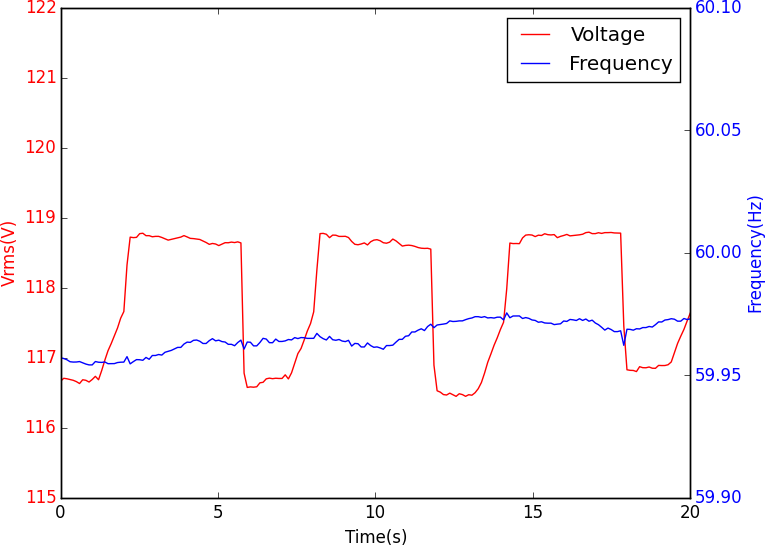
\includegraphics[width=0.9\linewidth]{img/hotplate.png}
	  \caption{Voltage signal produced by a hotplate.}
	  \label{intro:fig1:sub1}
	\end{subfigure}%
	\begin{subfigure}{.5\textwidth}
	  \centering
	  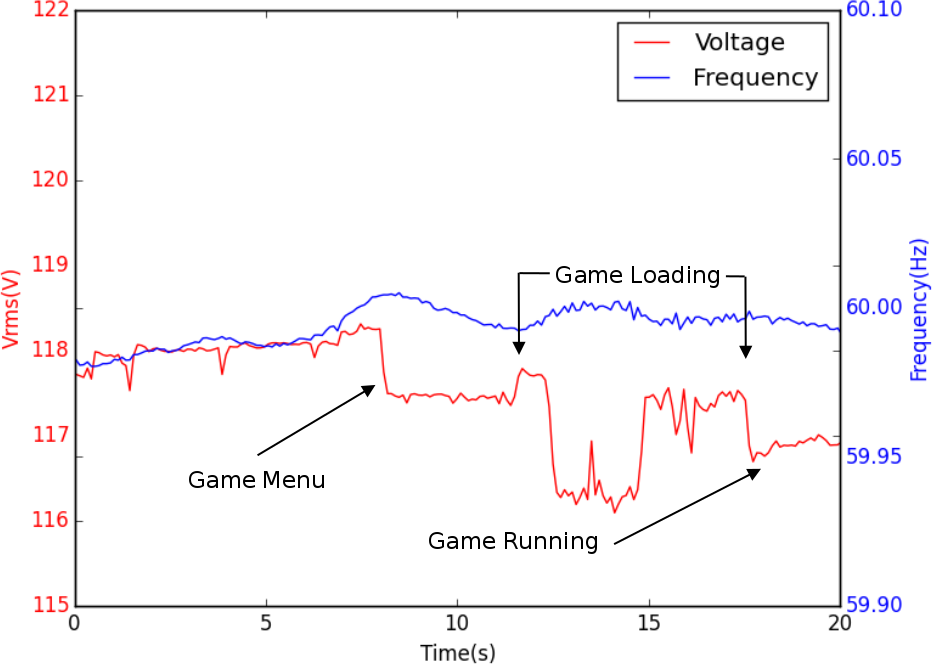
\includegraphics[width=0.9\linewidth]{img/PC.png}
	  \caption{Voltage signal produced by a desktop PC running a complex task}
	  \label{intro:fig1:sub2}
	\end{subfigure}
	
	\begin{subfigure}{1\textwidth}
	  \centering
	  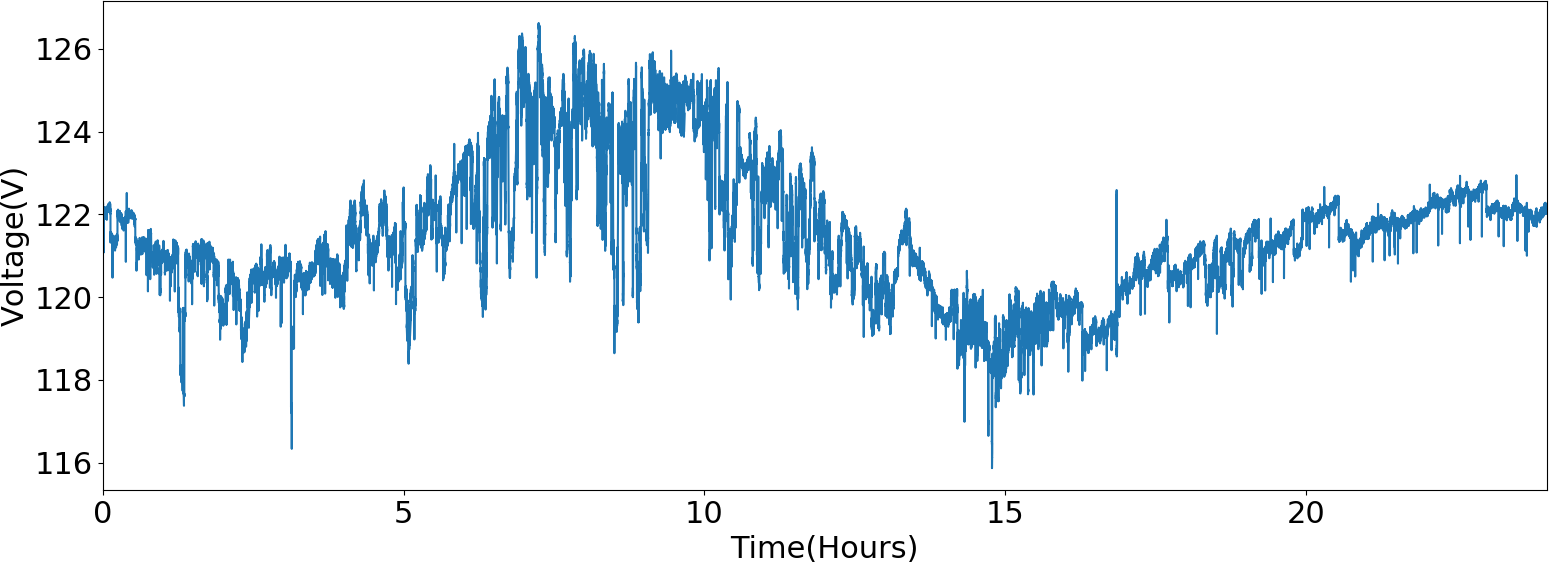
\includegraphics[width=0.9\linewidth]{img/johnson_daily.png}
	  \caption{Line voltage recorded over 24 hours in a residential household with photovoltaic installation.}
	  \label{intro:fig1:sub3}
	\end{subfigure}
	
	\caption{RMS voltage waveform generated form the consumer side of the meter under various conditions. All waveform were recorded using the OPQ Box 2.}
	\label{intro:fig:1}
\end{figure}

Residential power quality monitoring presents a number of issues. First of all, it is difficult to discern which side of the utility meter a power disturbance came from. Consider a voltage sag generated by a 1kW hot plate shown in Figure \ref{intro:fig1:sub1}.  Since the output impedance of the power grid is non-zero a high powered device can cause a significant voltage sag affecting every device connected to the same circuit. Secondly, recoding the voltage waveform resulting from non linear load can result in privacy leaks for the end user. Consider the voltage waveform produced by a PC running a video game as shown in Figure \ref{intro:fig1:sub2}. Throughout the game loading process the power load varies based on which components are in use. Furthermore, regions with CPU load, harddisk load and video card load can be readily identified by measuring the resulting voltage sag. Recording these event's has an adverse effect on end-users privacy and offers no immediate benefit in studying grid stability. Finally distributed power generation such as rooftop solar has significant effect on the residential voltage waveform. Consider the voltage waveform shown in Figure \ref{intro:fig1:sub3}. This waveform was recorded over 24 hours in a household with a rooftop photovoltaic installation. Similar to the voltage sag case since the power grid impedance is non-zero residential power generation will cause a voltage swell during peak hours of sunlight as evident by the waveform. Combined with the global voltage sag during hours of peak demand (3pm) combined with the lack of PV production during that time, photovoltaics installations can result in a daily $10V_{rms}$ swing. Residential power quality monitoring can be accomplished via a distributed sensor network made up of power quality monitoring devices with high degree of penetration across the end points of a power grid. Furthermore, in order to monitor the dynamics of the entire power grid via residential line voltage monitoring it is imperative to monitor across multiple locations simultaneously. This combined with temporal and spatial correlations of data produced by the sensors allows for identification of grid wide anomalies without a high rate of false positives. Additionally, not all power quality events affect the entire grid, due to the hierarchical structure of the power distribution. The final requirement for grid-wide monitoring is a novel distributed event detection system.

\section{Edge computing approach to power quality monitoring.}

IEEE1159 standard describes the techniques for single location power quality monitoring. For transient monitoring it suggests a sampling rate of at least 7680 samples/second, up to 1 Megasample/second. This implies that if a power quality event detection system relies on raw data from all monitors it would do so at a very large bandwidth cost. At 20 Ksamples/second at 16bit per samples a single monitoring device would generate 300Kb/second. Several thousand devices could easily saturate at 1Gb link with no obvious benefit. Collecting and recording all of the raw waveform data from residential power quality meters for batch processing presents some privacy concerns as outlined above. On board event detection methodology allows the measurement devices to select which temporal regions of measurements constitute an event. This is a perfect strategy from the consumer's perspective, since it would allow for recording of power quality information which directly impact their residence. As mentioned in Section \ref{intro:edge}, this method relies on a threshold based approach where every device has a computes several metrics from the raw waveform and compares then to preprogrammed threshold values. Metrics such as $V_{rms}$, fundamental frequency and THD are easily adapted for single point power quality measurements. Temporal regions during which these metrics surpass a threshold are considered by the device as a power quality event, and thus are recorded. 

The problem with the method outlined above is that grid-wide power quality events do not affect the entire grid in the same way. For example due to the grids hierarchical structure a voltage sag on one sub-circuit can manifest as as a sag of a different magnitude or even a swell on another.\cite{kahle2016power} This may result in a situation where some of the monitoring devices will not consider a power quality anomaly as an event, because it did not surpass the metric threshold, and simply ignore it. From the research perspective, however, it is important to get raw data from all of the affected devices not just the ones that were the most affected. This makes a hybrid centralized/decentralized event acquisition strategy more attractive for distributed residential power quality monitoring. In this scheme all monitoring devices use local processing resources to feature extract the incoming waveforms while storing them locally for several minutes. A sink collects all of the extracted features and looks for anomalies which are present in the feature data stream which we will refer to as triggering stream. If an anomaly is present in only a single device, it is highly probable that the disturbance occurred in the residence. Depending on the user's privacy preference, raw data for a single device anomaly can be be recorded for later analysis, or in case of a highly privacy conscious user, ignored. On the other hand if the triggering stream shows an anomaly temporally collocated across multiple devices, the entire network or a subset of the network may be queried for raw waveform data for a temporal region which corresponds to the disturbance in the triggering stream.

The main disadvantage of this method is that while there are plenty of power quality event detection methodologies for single location, there has been little development in the distributed event detection methods and metrics. Two problems are quite similar, indeed one may use the same metrics for distributed event detection as with the single point power quality monitoring. However, it's also important to consider temporal locality of anomalies detected across multiple devices and effects of device synchronization. Power quality anomalies such as voltage sags and transients will propagate through the transmission lines at the speed of light, however due to the non-linear elements which make up the power-line junctions, a certain temporal spread in event detection across multiple locations is expected. For large power grids such continental United States grids, large frequency fluctuations propagate in a highly nonlinear ways. In these cases the event propagation is limited by the inherent rotational inertia of the power generation systems, and the speed at which the grid protection elements such as reclosers and circuit breakers operate. Regardless, the closer local anomalies are detected in time, the more likely are they to be a result of a gridwide event. Unfortunately, it is unfeasible to perfectly temporally synchronize the distributed power quality monitors. While methods such as GPS can in principle provide synchronization of up to 10ns jitter across a large geographical region, they require a line of sight to the sky, and add a non-trivial cost to the bill of materials for every power quality meter. Furthermore, GPS is prone to losing signal depending on atmospheric conditions, and can be very sensitive to fluctuations in the power supply voltage, a critical time in power anomaly detection. An alternative to GPS is Network Time Protocol. Network time protocol can provide timing synchronization on the order of $~10ms$ across Internet, which is on the order of $\frac{1}{2}$ of a grid cycle. NTP performance could be further improved by using geographically close time servers which are themselves synchronized via GPS. Consider a situation where two devices are located in household which experience a local $100ms$ power quality disturbance every $10$ minutes. Even with a $~10ms$ synchronization jitter, it will take on average $21.5$ days before the two disturbances are observed within $20ms$ of each other. If a third device is introduced, it is highly unlikely that all 3 would observe unrelated local anomalies within $20ms$ of each other over the lifetime of the power quality monitoring network. This implies that combination of temporal and threshold based correlation on the feature extraction data would allow one to build a robust residential based power grid monitoring system which would yield a very low rate of false positives. 

\begin{figure}[h]
	\centering
	  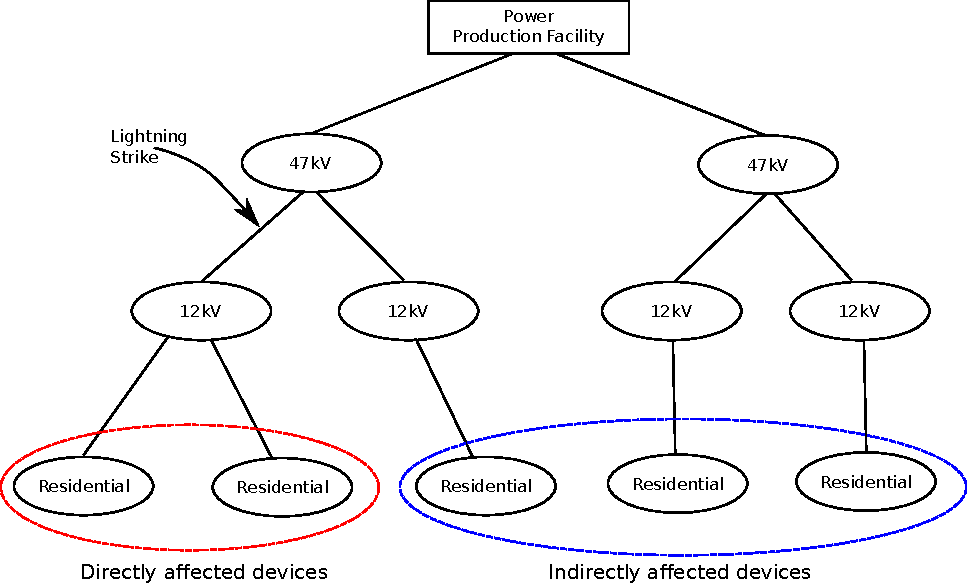
\includegraphics[width=0.9\linewidth]{img/grid_hierarchy_cartoon.pdf}
	  \caption{Power quality anomaly propagation example.}
	  \label{intro:fig2}
\end{figure}

\section{Thesis claim and evaluation} \label{intro:sec:claim}

Today's big data world is plagued with the issues of data cleaning and validation, even though it's being relied on for timely, accurate and actionable intelligence. With large ingress of unstructured data these issues are unavoidable, and preprocessing will remain a large portion of the analysis workload. However, in the case of sensor networks designed for a specific purpose, the tasks of anomaly detection can be pushed to the edge of the network using the Napali methodology. The claim of this thesis is that Napali provides novel architecture that is both a feasible solution to the problem of distributed power quality monitoring and which also provides significant benefits over the two standard alternative architectures (all computation/storage at nodes, all computation/storage at the sink).

To evaluate the feasibility of the Napali framework, I propose to implement it as part of the Open Power Quality(OPQ) system and apply it to the problems of power quality monitoring. Combined with higher level anomaly analysis, Napali provides important services for a Open Power Quality power quality monitoring network. This network is made up of a group of monitoring devices as well as a centralized data sink server. This system will be deployed for testing at the University of Hawaii at Manoa campus, by deploying power quality monitors across at least 20 buildings on campus. The University of Hawaii at Manoa campus is a unique testbed for such a network, since entire campus is isolated to its own microgrid, connected to the municipal Oahu grid via a 46kV feeder. Furthermore, the University of Hawaii has deployed a set of smart power monitors at the key positions in the grid, which can be used as a state of the art ground truth for evaluation of OPQ performance. 

The system relies on a custom residential power quality monitor called OPQ Box, designed specifically for distributed monitoring using the Napali framework. Instead of performing local analysis on the voltage waveform with the aim of PQ anomaly detection, or forwarding all the recording measurements to the centralized sink, OPQ boxes computes a small subset of features on the input voltage waveform. These features are then forwarded to the Napali framework's centralized sink which performs the anomaly detection on reduced data, while the raw waveform is retained for a short time on the OPQ Box. If the sink determines that a possible anomaly has occurred, a request is sent to the affected and nearby devices for raw data.

The goal of Napali is not to provide a low rate of false positives for a particular type of a power quality disturbance. Indeed, once the raw data is acquired by the sink, filtering through the potential anomalies is trivial using well established methods. Instead, the focus of my detection system is balancing low bandwidth required for detection with the low rate of false negatives. Furthermore, monitoring at the leaf edges relies on the hierarchical nature of the power grid in order to ascertain the state of the entire power generation and delivery system. As noted in the literature, power quality disturbances tend to propagate down the hierarchy as shown in Figure \ref{intro:fig2}. 

Consider a lightning strike on a hypothetical 12kV feeder line in a hierarchical power grid. The directly affected devices will be the ones downstream from the disturbance. These devices will experience the most severe effects, most notably transients, as they propagate throughput the power delivery infrastructure. The indirectly affected devices will expedience a power anomaly mainly attributed to the power production entities trying to compensate for the large disturbance caused by the lightning strike. Thus, monitoring of the leaf edges of the power delivery system can in principle provide insights into the disturbances that originate deep inside the power distribution network.

The Open Power Quality system is designed to be a test bed for development of new power quality detection and analysis algorithms. Its introduction will facilitate development of new techniques and methods for studying power system, by utilizing the Napali framework as the main anomaly detection methodology. To evaluate the benefits of this architecture, I will assess the data collected by the OPQ network at the University of Hawaii in order to determine if the claimed benefits of the architecture are observed in practice. The description of the evaluation processes for the benefits described in Section \ref{intro:section:napali} are summarized below.

\begin{enumerate}
  \item \textbf{Bandwidth usage is minimized:} Bandwidth consumption of the OPQ system will be carefully monitored, recorded and compared to the bandwidth required to transmit the equivalent amount of raw data. A more detailed description of this evaluation can be found in Section \ref{iexp:sec:band}.
    
	\item \textbf{Effects of latency are minimized:}  Latency limits of the triggering system will be examined. Since these are heavily dependent on the raw data storage ability of the OPQ Box, latency effects will be tested under various amount of memory allocated for this task. A more detailed description of this evaluation can be found in Section \ref{iexp:sec:lat}.
  
  \item \textbf{Temporal locality:} Data acquired from the UH building level meters will be compared with the data acquired via the Napali triggering framework.  This will allow me to establish the rate of false positives and negatives and evaluate the temporal locality triggering algorithm. Furthermore, the single location events, which are normally rejected by Napali will also be examined and compared to the data provided by the building power meters. A more detailed description of this evaluation can be found in Section \ref{iexp:sec:loc}.

  \item \textbf{Sink processing requirements are minimized:} Synthetic benchmarks will be carried out on the sink node to determine the scalability of the triggering system. These scalability metrics will be compared with a synthetic benchmark of running multiple copies of the OPQ Box analysis software on the same node. This will allow me to compare the scalability of the sink node in the case of sending the entirety of raw data stream versus the Napali frameworks approach of only sending extracted metrics. A more detailed description of this evaluation can be found in Section \ref{iexp:sec:scale}.

	\item \textbf{Sub-threshold data acquisition:} Evaluation of the sub-threshold data acquisition will performed in two ways. First, the triggering stream from the OPQ Boxes will be stored along with the acquired raw data. The triggering stream can be used to compute which fraction of devices would have self triggered if operating autonomously. Next the building level meters self triggering capabilities, will be compared to the Napali, sub-threshold triggering in order to compare Napali to a commercially deployed system. A more detailed description of this evaluation can be found in Section \ref{iexp:sec:sub}.
  
\end{enumerate}
Although power failure resiliency and flexible privacy are claimed benefits of the Napali architecture, they will not be evaluated as part of this thesis research. Flexible privacy would require a much larger deployment, and a user study, which is beyond the scope of this project. Furthermore the power failure resilience of the Napali framework would require a significant development effort in development of the battery management system. Since complete power failures are quite rare, there is no guarantee that a single power outage would occur at the UH campus during the deployment. 

The last claim of this dissertation is that the Napali architecture can be applied to other domains. Once the Napali framework is fully characterized, and its strengths and weaknesses are well understood, I intend to perform an in-depth literature review of other domains which could benefit from Napali-like approach to event detection. I will also characterize the kinds of design changes to existing sensors that the Napali Framework will require in order to apply it to these domains.



\chapter{Related Work}


- wavelet compression
- fourier compression
- power quality 



\chapter{OpenPowerQuality}
\begin{figure}[h]
  \begin{center}
  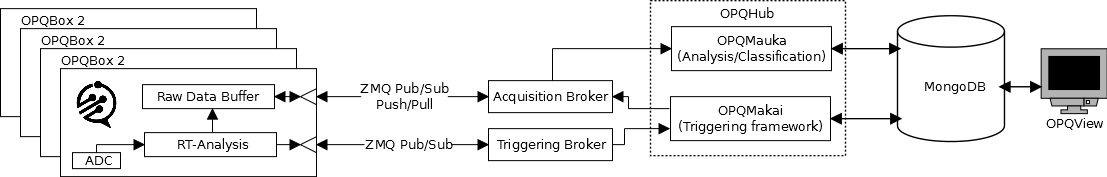
\includegraphics[width=0.9\textwidth]{img/system-diagram.png}
  \end{center}
  \caption{Block diagram of the OPQ Power Quality monitoring system.}
  \label{fig:1}
\end{figure}

OpenPowerQuality(OPQ) power quality monitoring network utilizes residential power quality meters, called OPQBoxes, in order to detect anomalies in the electricity distribution accross the Oahu power grid. In addition to OPQBoxes, OPQ project utilizes a cloud based aggregation services for power quality event detection, classification and display. The block diagram of the OPQ network is shown in Figure \ref{fig:1} .

The major components of OPQ are:
\begin {itemize}
	\item OPQBox: in-house designed, open source power quality meter.
	\item Makai: data aggregation and event detection service.
	\item Mauka: event analysis and classification service.
\end {itemize}

Following sections describe the OPQ network components, services and protocols.

\section{OPQBox}

OPQBox is an in-house designed power quality meter which focuses on providing the means for cheap, extensible and accurate residential power quality measurements. The block diagram of the current revision of OPQBox, OPQBox2 is shown in the Figure \ref{fig2:sub1}. A complete device in an acrylic enclosure is shown in Figure \ref{fig2:sub2}.

\begin{figure}[h]
	\centering
	\begin{subfigure}{.5\textwidth}
	  \centering
	  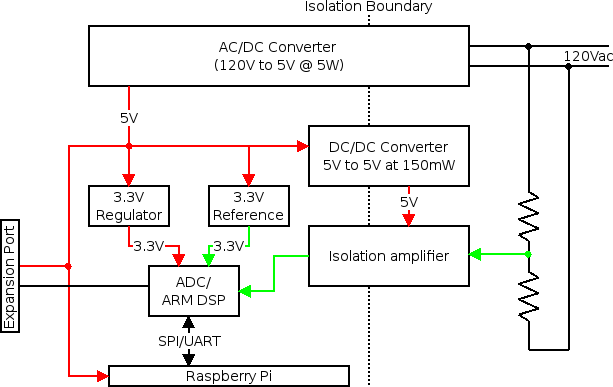
\includegraphics[width=0.9\linewidth]{img/opqbox_diagram.png}
	  \caption{OPQBox2 Block Diagram. The power path is in red, signal path is in green and the digital IO is in black.}
	  \label{fig2:sub1}
	\end{subfigure}%
	\begin{subfigure}{.5\textwidth}
	  \centering
	  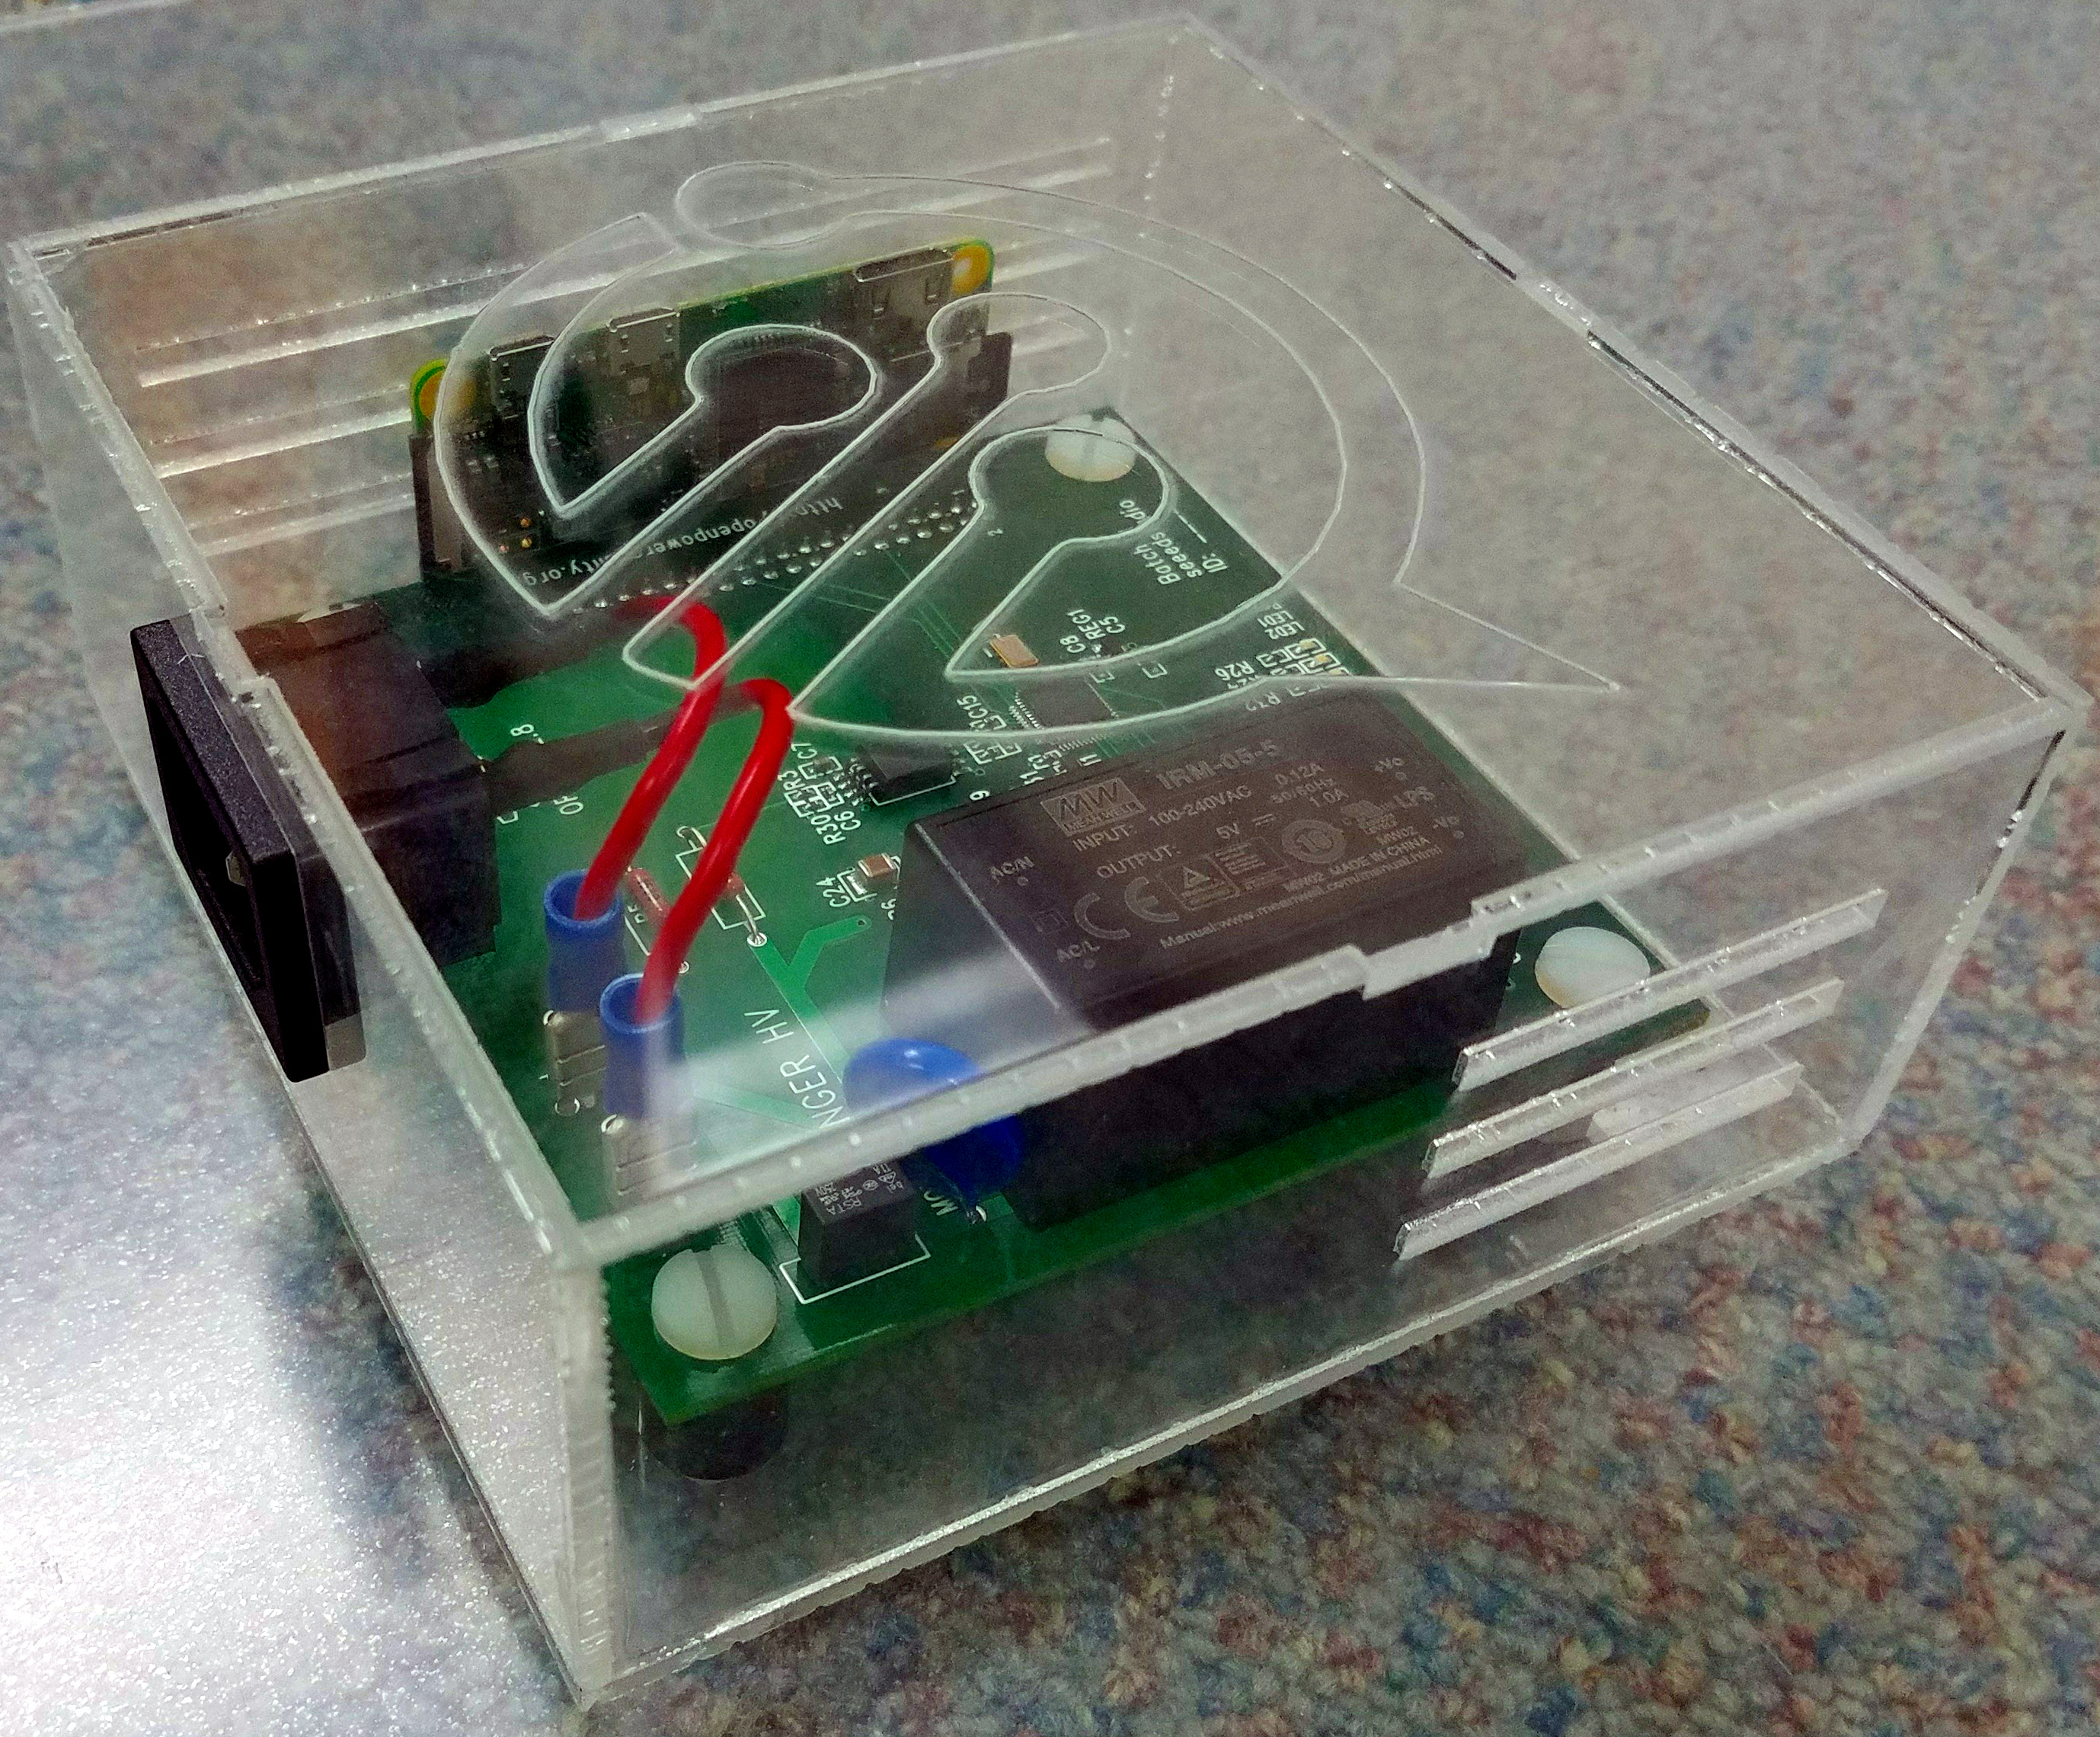
\includegraphics[width=0.7\linewidth]{img/opqbox_photo.jpg}
	  \caption{OPQBox2 in an acrylic enclosure.}
	  \label{fig2:sub2}
	\end{subfigure}
	\caption{(a)OPQBox2 block diagram and (b)production OPQbox ready for deployment}
	\label{fig:2}
\end{figure}

The power system of the OPQbox2 electrically isolates most of the device from the AC mains power. An isolated AC-DC converter generates $5V_{dc}$ from the mains $120V_{ac}$. 5V is used to power the Raspberry Pi, equipment connected to the expansion port, 3.3V regulators and voltage reference and an isolated DC/DC converter. 3.3V is used to power the isolated end of the isolation amplifier as well as the STM32F3 analog to digital converter/digital signal processor(ADC/DSP). The hot side of the isolation amplifier is powered from the isolated DC/DC converter. This allows OPQbox to function with the battery attached to the expansion port, so that it may retain data and continue to operate during a power outage. 

The analog signal path of the OPQBox2 is complicated by the fact that the STM32F3 ADC/DSP is electrically isolated from the mains power. Previous iteration of the OPQBox, OPQBox1, overcame this by employing small circuit board mount isolation transformer. Unfortunately it was found that the frequency response of these transformers varied wildly between individuals, thus incurring a lengthy calibration process for each device. Design on the OPQBox2 solved this issue by using an AMC1100 isolation amplifier as the isolation component. Internally AMC1100 consists of a single die comprised of a $\Sigma\Delta$ analog to digital and digital to analog converters. These converters are separated by a silicon glass region on the integrated circuit which acts as a coupling capacitor. Since the signal passes the isolation boundary as a $\Sigma\Delta$ encoded digital signal, it incurs no distortion and no additional calibration is required. In order to match the dynamic range of the AMC1100 the $120V_{ac}$ is passed through the resistor divider to attenuate it to $120mV_{ac}$. The input and output of the isolation amplifier is filtered with a passive first order anti-aliasing filter. Isolated signal is then digitized via a 16bit ADC of the STM32F3 DSP at $12 KSps$, which gives 200 data samples per grid cycle. Internally digitization process runs asynchronously with the respect to the the DSP CPU, in order to minimize timing jitter. It was verified that the sampling jitter of the ADC is less then 1us, however due to limited precision of equipment an exact figure was not established. Data stream in its digital form is transfered to the Raspberry Pi single board computer(SBC) for analysis.

\begin{figure}[h]
  \begin{center}
  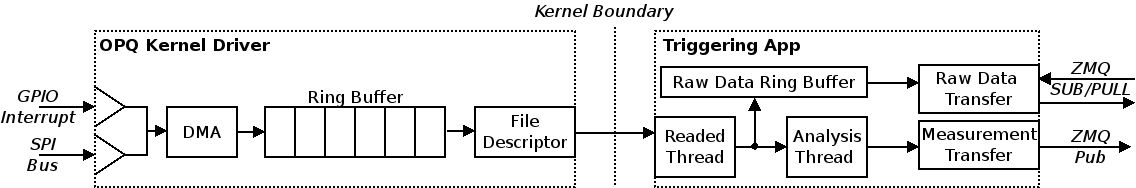
\includegraphics[width=0.9\textwidth]{img/opqbox_software.png}
  \end{center}
  \caption{Block diagram of the OPQBox2 software stack.}
  \label{fig:3}
\end{figure}

Raspberry Pi SBC is responsible for signal analysis and anomaly detection. Raspberry Pi model used in OPQBox is the Pi Zero W equipped with 256MB of main memory and a single core 1GHz ARM11 CPU. Furthermore Pi Zero W is equipped with an on-board 802.11n WIFI transceiver, which removes the need for an external WIFI dongle used in previous OPQBox devices. Software stack of the Raspberry Pi aims to deliver a full featured power quality analysis framework despite it's the rather limited hardware capabilities. A block diagram of the software stack is shown in figure \ref{fig:3}. Digital data is transfered from the DSP to the Raspberry Pi via Serial Peripheral Interface, with the Pi acting as the master and the DSP as a slave device. A hardware interrupt line is used to inform Pi software that the DSP is ready for the data transfer. During the initial design of the OPQbox2 software, SPI data transfer was attempted in userland. However due to the lack of support for DMA in the SPI kernel-to-userland bridge, a large portion of the CPU time was spent facilitating data transfer, resulting in degraded analysis performance as well as missed data samples. Current revision of the OPQBox2 software stack utilizes a kernel driver for management of SPI bus. Internally OPQ driver maintains a ring buffer of 16 windows each 200 data samples in size. Upon the receiving the interrupt for the DSP, the CPU sets up the DMA transfer and the DMA engine transfers a 200 sample window into the kernel memory without CPU interaction. This scheme requires the CPU to only service 60 interrupts a second, with each interrupt requiring on the order of 100 instructions, yielding the CPU utilization of less then $1\%$ in normal operation. Userland applications communicate with the kernel driver using a file descriptor, where every $write$ system call yields 200 samples of raw waveform. Thus the smallest window that a userland application will process is a single AC cycle of the grid mains.

Userland component of the OPQBox2 software is a milti-threaded extensible analysis framework called Triggering. The reader thread is responsible for transferring and accumulating data from the kernel driver. The smallest data buffer that the Triggering application processes at any given time is 10 grid cycles or 2k samples. Once the cycles are transfered to the userland and timestamped, they are passed to the analysis thread for feature extraction, as well as to the Raw Data Ring Buffer(RDRB). Since internally all data is addressed using shared pointers so during data duplication no copying is required. RDRS is capable of buffering up to an hour of historic data before it's overwritten resulting in the RDBS maximum size of 100MB. 

Analysis thread of the Triggering application performs feature extraction of the raw data windows of 2000 samples. At the moment only two metrics are calculated:
\begin{itemize}
	\item Fundamental frequency.
	\item RMS Voltage.
\end{itemize}
Fundamental frequency is calculated by computing the zero crossings of the AC waveform. Since a sinusoid will have two zero crossings for a full cycle the frequency can be calculated as:
\begin{equation} \label{eq:1}
 f = \frac{1}{\frac{2}{n}\sum\limits_{k=0}^{k=n}{\Delta t_{k}}}  
\end{equation}

\begin{figure}[h]
	\centering
	\begin{subfigure}{.5\textwidth}
	  \centering
	  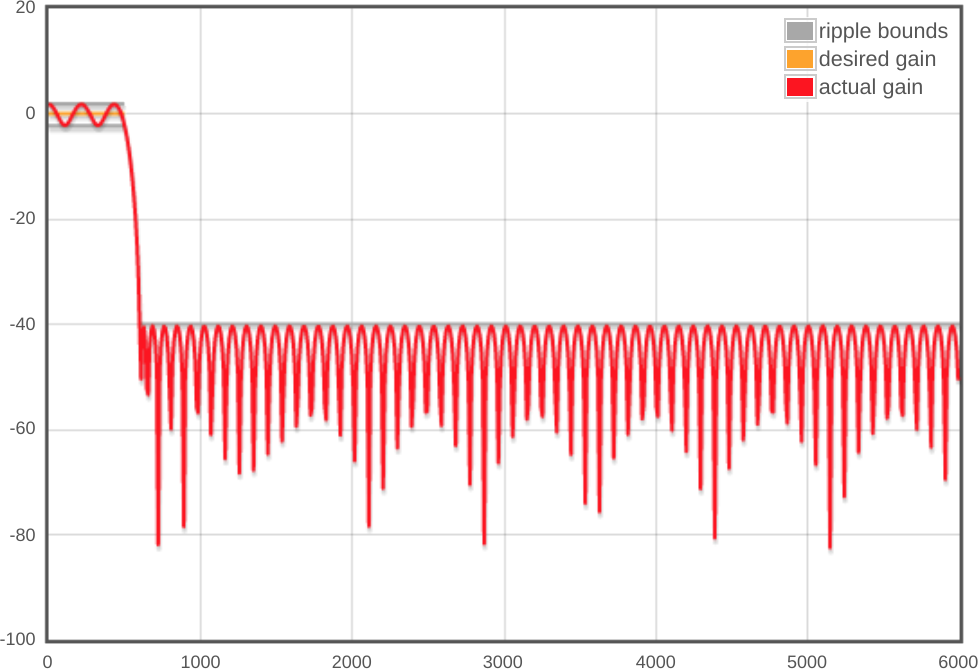
\includegraphics[width=0.9\linewidth]{img/filter1_gain.png}
	  \caption{}
	  \label{fig4:sub1}
	\end{subfigure}%
	\begin{subfigure}{.5\textwidth}
	  \centering
	  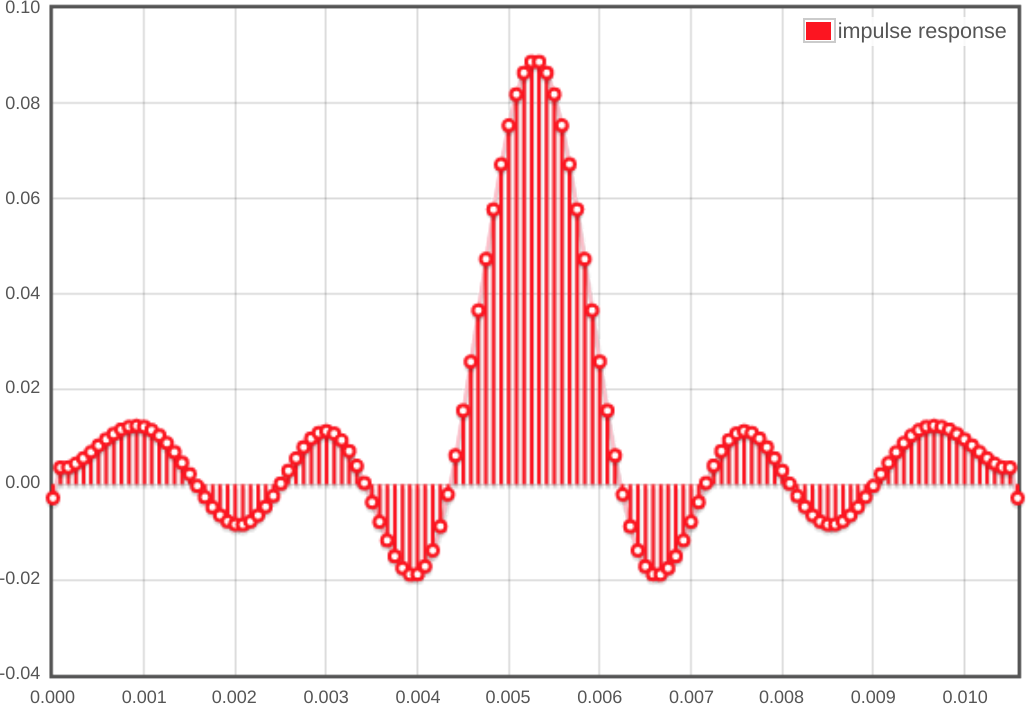
\includegraphics[width=0.9\linewidth]{img/filter1_response.png}
	  \caption{}
	  \label{fig4:sub2}
	\end{subfigure}

	\begin{subfigure}{.5\textwidth}
	  \centering
	  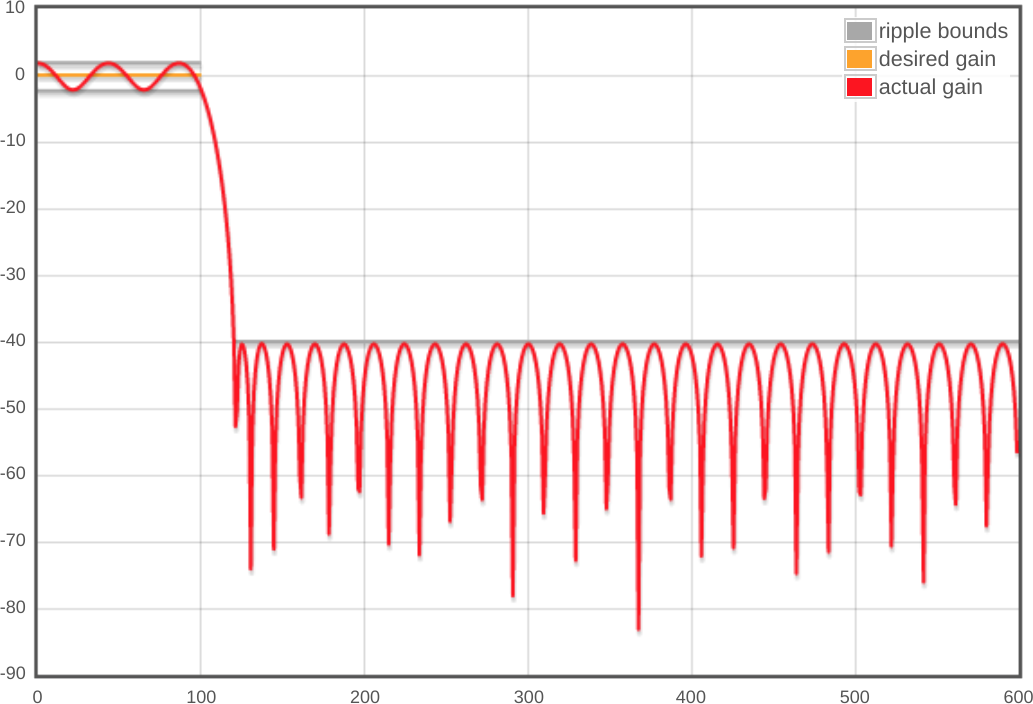
\includegraphics[width=0.9\linewidth]{img/filter2_gain.png}
	  \caption{}
	  \label{fig4:sub3}
	\end{subfigure}%
	\begin{subfigure}{.5\textwidth}
	  \centering
	  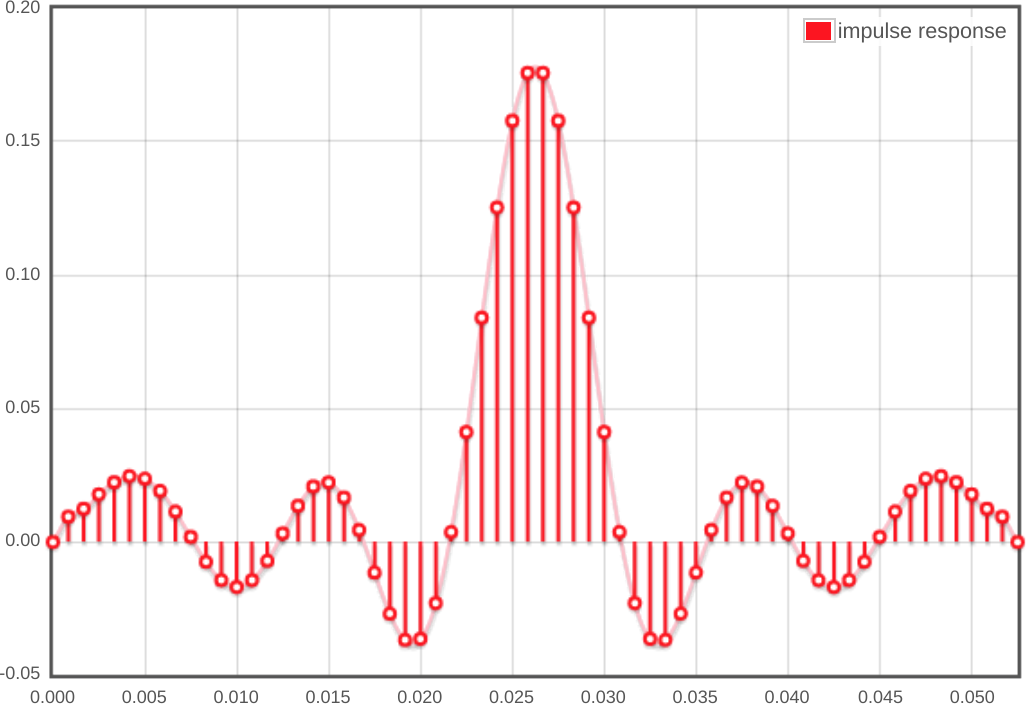
\includegraphics[width=0.9\linewidth]{img/filter2_response.png}
	  \caption{}
	  \label{fig4:sub4}
	\end{subfigure}
	\caption{Filters used for mains frequency calculation. (a)Downsampling filter gain. (b)Downsampling filter impulse response. (c)Lowpass filter gain. (d)Lowpass filter impulse response.}
	\label{fig:4}
\end{figure}

Where the $\Delta t_{k}$ is the k'th time between two adjacent zero crossings. In order to improve the accuracy of the frequency calculation one must first filter out as much of out of phase noise as possible. Since our sampling rate is quite high(12kSps) and the fundamental frequency is quite low (60Hz) it is very computationally expensive to perform this filtering in a single step. Instead filtering is accomplished via a set of two finite impulse response(FIR) filters shown in Figure \ref{fig4:sub2} and \ref{fig4:sub4}. First the Down sampling filter is applied to the raw waveform, which results in the frequency response shown in Figure \ref{fig4:sub1}. As is evident by the plot the frequency content of the result is 0-600Hz, Thus it can be downsampled to the $\frac{N}{10}$, or 200 samples without aliasing. Next the low pass filter is applied to the downsampled waveform with the frequency response shown in Figure \ref{fig4:sub3}.This resulting frequency content is 0-100Hz, thus all of the higher frequency harmonics and noise are removed. Finally the twice filtered downsampled waveform is used to estimate the fundamental frequency according to the Equation \ref{eq:1}. The zero crossings themselves were calculated by using linear interpolation between two points which bracket the time axis.

In order to verify the error in our frequency measurement, a function generator(SIGLENT SDG1025) was used to inject a $60Hz$ $120mV_{pp}$ superimposed with $1\%$ white noise into the input of the AMC1100 anti-aliasing filter, bypassing the voltage divider. The resulting frequencies were calculated and recorded by the OPQBox2 and histogramed as shown in Figure \ref{fig5:sub1}. It was found that the OPQBox2 overestimated the frequency by $300\mu Hz$ with $\sigma  = 230\mu Hz$. All electrical generation systems connected to the grid run syncroniously with each other, meaning that while small variations in voltage are common across locations, the fundamental frequency and phase must remain strictly in sync. This effect is demonstrated in Figure \ref{fig5:sub2}, which is a frequency fluctuation event recorded on November 8 2017. While the two devices were separated by ten miles, their frequency measurements track closely together.

\begin{figure}[h]
		\centering
	\begin{subfigure}{.5\textwidth}
	  \centering
	  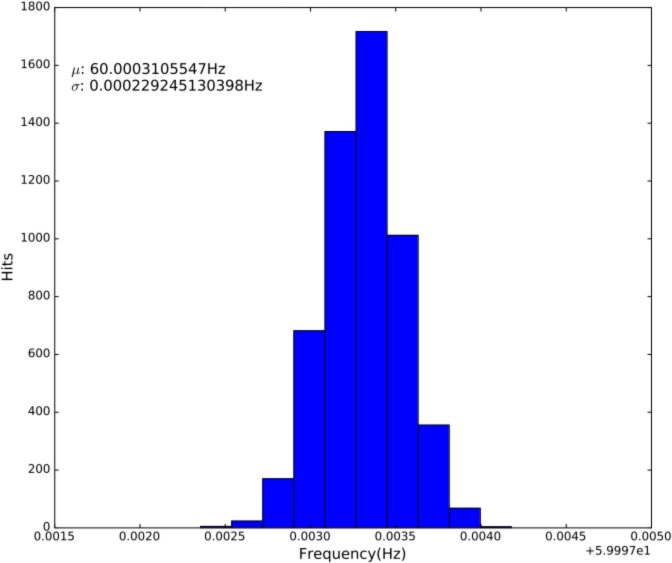
\includegraphics[width=0.9\linewidth]{img/frequency_verification.png}
	  \caption{}
	  \label{fig5:sub1}
	\end{subfigure}%
	\begin{subfigure}{.5\textwidth}
	  \centering
	  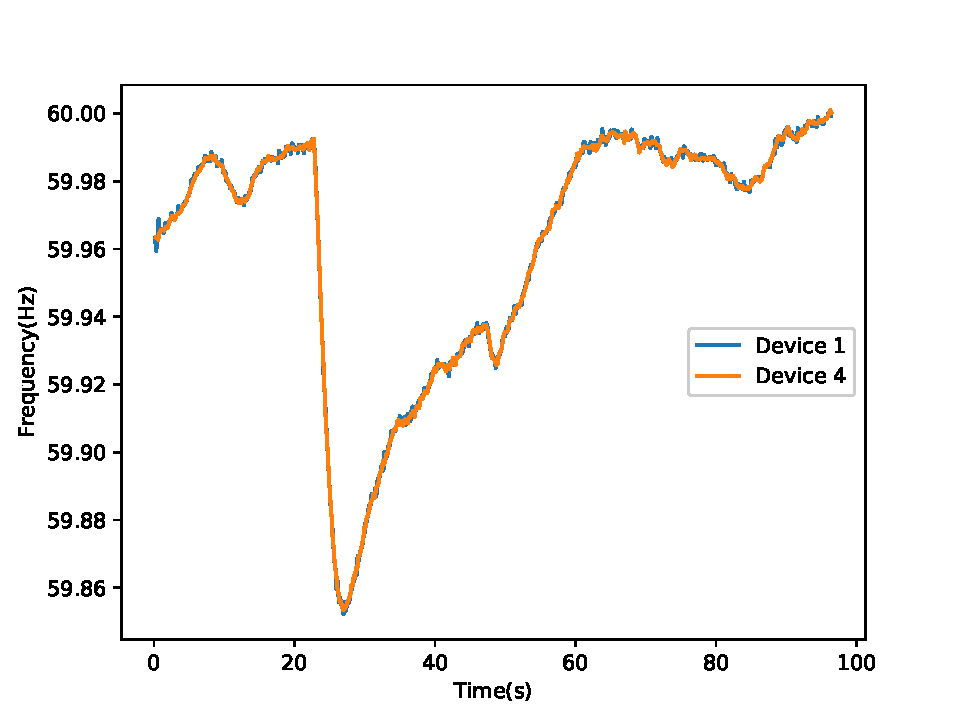
\includegraphics[width=1.1\linewidth]{img/frequency_two_devices.pdf}
	  \caption{}
	  \label{fig5:sub2}
	\end{subfigure}
	\caption{Filters used for mains frequency calculation. (a)Downsampling filter gain. (b)Downsampling filter impulse response. (c)Lowpass filter gain. (d)Lowpass filter impulse response.}
	\label{fig:5}
\end{figure}

Root mean square voltage($V_{rms}$) in electrical power is the equivalent value of DC voltage which would dissipate the same power in the resistive load. $V_{rms}$ is a convenient measure for detecting voltage sags and swells, since they result in nominally higher and lower computed value. For the sinusoidal signal $V_{rms}$ can be calculated from the peak to peak value($V_{pp}$) as:
\begin{equation} \label{eq:2}
	V_{rms} = \frac{V_{pp}}{2\sqrt{2}}
\end{equation}
It is common for multimeter to employ the equation above for computing $V_{rms}$. However this equation will only work for a perfect sinusoid, and thus does not result in a suitable metric for identifying power quality disturbances. Instead OPQBox2 computes $V_{rms}$ as follows:
\begin{equation} \label{eq:3}
	V_{rms} = \sqrt{\frac{1}{n}\sum\limits_{k=0}^{k=n}V_{k}^{2}}
\end{equation}
Similarly to the frequency calculation OPQBox2 will use a 10 cycle window for a single $V_{rms}$ calculation, however unlike the frequency calculation the input is not filtered a priori. An example of a power quality disturbance which exhibits low $V_{rms}$ is shown in Figure \ref{fig6:sub1} and \ref{fig6:sub2}. These disturbances are the result of a lighting strike recorded by two OPQBox2 devices on Nov 1, 2017.

\begin{figure}[h]
		\centering
	\begin{subfigure}{.5\textwidth}
	  \centering
	  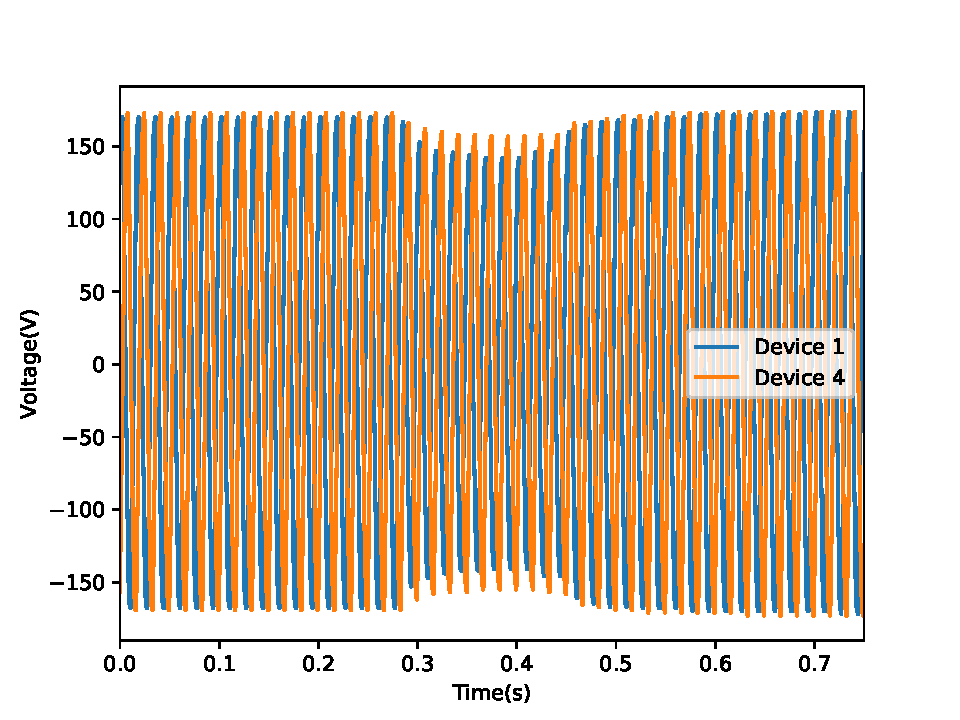
\includegraphics[width=0.9\linewidth]{img/voltage_sag.pdf}
	  \caption{}
	  \label{fig6:sub1}
	\end{subfigure}%
	\begin{subfigure}{.5\textwidth}
	  \centering
	  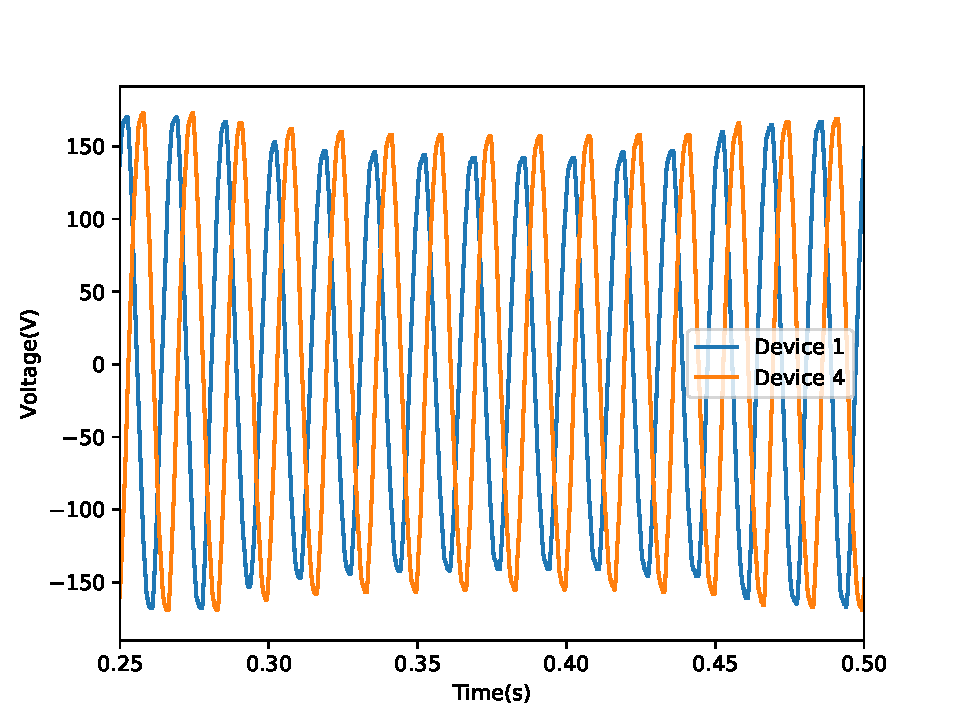
\includegraphics[width=0.9\linewidth]{img/voltage_sag_zoomed_in.pdf}
	  \caption{}
	  \label{fig6:sub2}
	\end{subfigure}
	\caption{A lightning strike recorded by two OPQBox2 devices separated by 10 miles. (a)A lightning strike manifested as $V_{rms}$ dip which lated 11 cycles. (b) As a consequence of using NTP these devices have $\frac{1}{2}$} cycle mismatch in reported timestamps.
	\label{fig:6}
\end{figure}

Computed fundamental frequency and $V_{rms}$ are transmitted to the Makai service for aggregation. Data transmission is handled using 0MQ software stack with Curve25519 elliptic curve encryption. Each device holds a unique of private and public keys, as well as the servers public key, allowing both the Makai service and the OPQBox2 to verify it's peer. Internally metrics transmission uses 0MQ's PUB/SUB protocol. This protocol is a publish subscribe one to many topology, with each message containing the topic, and a payload. Additionally 0MQ pub-sub topology allows for multiple sub peers with subscriptions forwarder to the publisher automatically via a side channel. This allows for the aggregation service to be spread across multiple nodes, with minimal network overhead.

If the aggregation service determines that an anomaly has occurred, it is able to request raw waveform from the OPQBox2 RDRB via a separate 0MQ pub sub channel. If the RDRB buffer contains data for the requested temporal range, OPQBox2 will send the available data to the aggregation service via a push pull 0MQ channel. Protobuf message serialization is used to encode messages across the OPQ ecosystem. 

In order to make a distributed measurement, all of the OPQBoxes on the OPQ network need to maintain an accurate time reference. Time synchronization across multiple OPQBoxes is accomplished using the Network Time Protocol. The expansion port of the OPQBox2 supports a GPS receiver, however using it is detrimental to the OPQBox2 utility. GPS receivers require line of sight to the sky, and since the with out on-board real-time clock, every power interruption requires a GPS cold start. NTP performance has been verified against GPS resulting in time error of $8ms\pm 5ms$ which is typical for NTP running over the Internet with a close by NTP server. This error is visualized in a Figure \ref{fig6:sub2}. With a large coincidental $V_{pp}$ drop across two devices, a 7ms phase error is clearly visible.

\section{OPQ Makai}

OPQ Makai is a distributed extensible microservice framework responsible for receiving the triggering stream from the OPQBoxes, locating anomalous temporal regions and requesting raw waveform for the anomalous time ranges. As evident from the block diagram shown in Figure \ref{fig:7}, Makai consists of three major components: Acquisition Broker, Triggering Broker, and the Acquisition Service. 
\begin{figure}[h]
  \begin{center}
  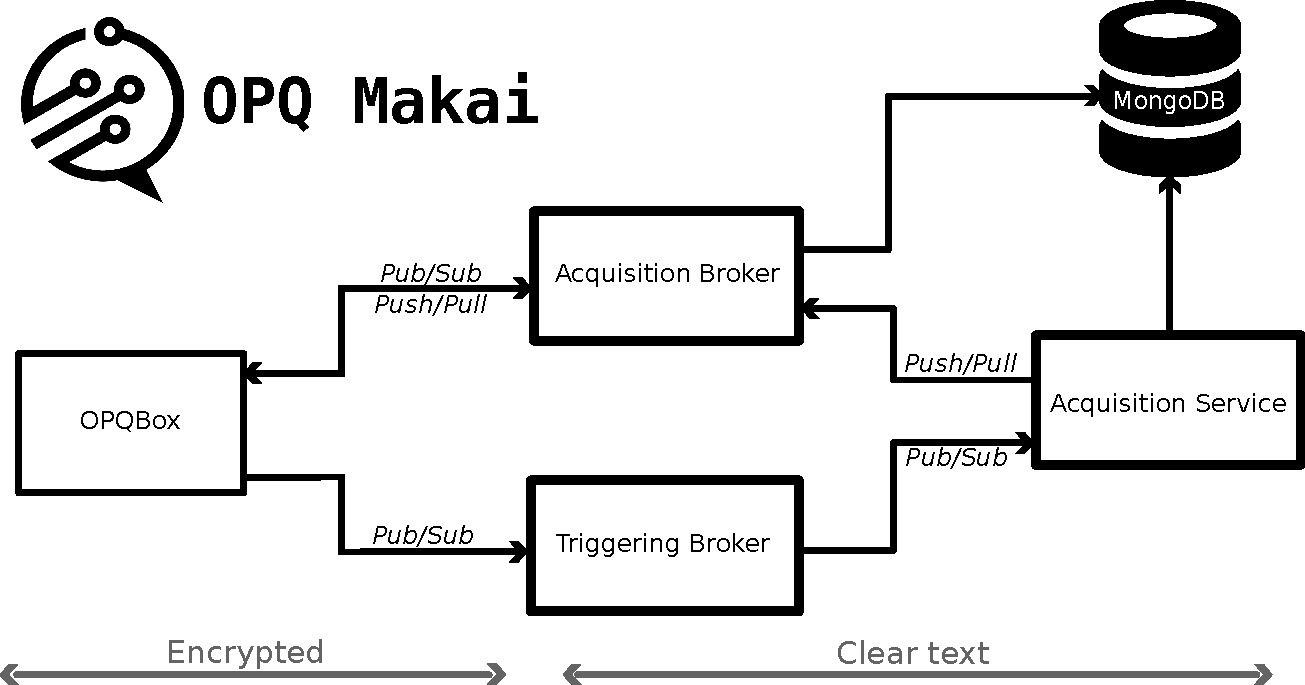
\includegraphics[width=0.6\textwidth]{img/makai_main.pdf}
  \end{center}
  \caption{Block diagram of the OPQ Makai.}
  \label{fig:7}
\end{figure}

\subsection{Triggering Broker}

Triggering Broker is perhaps the simplest component of the OPQMakai system. The triggering stream generated by the OPQBoxes is encrypted to preserve users privacy. In order to minimize the CPU time spent decrypting the data across multiple opq services, Triggering Broker is used to decrypt the data and send clear text measurements across the rest of the OPQHub ecosystems. Triggering Broker uses the 0mq sub socket to receive data form OPQBoxes, and send, it via a pup socket to any connected client. Another potential role of the Triggering Broker is load balancing. Since the 0MQ pub/sub sockets are subscription based, services connecting to the triggering broker can selectively receive measurements only from boxes they are interested in. 

\subsection{Acquisition Broker}

Acquisiton Broker manages the two way communication between the OPQBoxes and the rest of the cloud infrastructure. Unlike the triggering stream which originates from the OPQBox, two way communication is always initiated by the cloud services. Two way communication is realized via a command response interface, where the opq service initiates the communication by sending in clear text command to the Acquisition Broker, which then forwards it in the encrypted form to the appropriate OPQBoxes. There are three command types which can be handled by the Acquisition Broker:
\begin{itemize}
\item{\textbf{(PING)Ping:}} The ping command is broadcast periodically across all of the OPQBoxes, in order to monitor the health of the OPQ network. The OPQBox response to this command contains diagnostic information, such as the timestamp of the last event requested, ip address and the name and strength of the WIFI network the OPQBox is connected to.
\item{\textbf{(CMW)Change measurement window:}} This command allows to vary how often a triggering stream message is generated and delivered to the triggering broker. This is accomplished by varying the length of the temporal window used to derive the triggering metrics. This allows the OPQ system to analyze a finer grained measurements if a potential anomaly is taking place. 

\item{\textbf{(RD)Send raw data:}} This command instructs the OPQBox to send data from the its raw data buffer to the cloud. 
\end{itemize}

The last command in particular is unique, because it's response is trapped by the acquisition broker, as opposed to being passed to the agent which initiated communication. In this case the raw data is serialized and stored in the mongo database. Furthermore, Acquisition Broker notifies all connected agents that a new anomaly has been recorded via a 0mq pub message.

\subsection{Acquisition Service}

Acquisition Service middleware that resides in between the Triggering and Acquisition Brokers. It processes the triggering stream and manipulates it using the \textbf{CMW} command and if an anomaly is suspected requests raw data from boxes via the \textbf{RD} command. The Acquisition Service app itself does not perform any analysis of the triggering stream. Instead it provides a loadable plugin interface which allows for a runtime hotplugable analysis. Since the OPQMakai core is written in the rust programing language, the loadable object interface supports supports any programing language with LLVM bindings. As such OPQMakai plugins can be developed in C/C++, Rust, or even Lisp. Currently three plugins are implemented:

\begin{itemize}
\item{\textbf{Print Plugin:}} Prints the triggering stream to the stdout for debugging purposes. 
\item{\textbf{Ketos:}} A Lisp interpreter built on top of the LLVM for manipulating/debugging the triggering stream.
\item{\textbf{Threshold:}} This plugin monitors the triggering stream, while looking for metrics which exceed the user defined thresholds. If the threshold is crossed, data from all of the OPQBoxes is requested for the offending time interval via the RD command.
\end{itemize}

Future revisions of Acquisition Service will likely include a python interpreter plugin, however due to the persistent global state in the python interpreter only a single python instance can run in the given address space.

\section{OPQMauka}
OPQMauka service is responsible for higher level classification and filtering of the anomalies generated by the OPQMakai. Since anomalies generation only
relies on the triggering stream features and not raw data, OPQMakai is not able to ascertain if the anomaly is an actual power quality event, event type, or its severity. OPQMauka on the other hand operates on the raw data, thus it is able to perform high level analysis to meet industry standards for vent classification. The block diagram of the OPQ Mauka is shown in \ref{fig:8}.
\begin{figure}[h]
  \begin{center}
  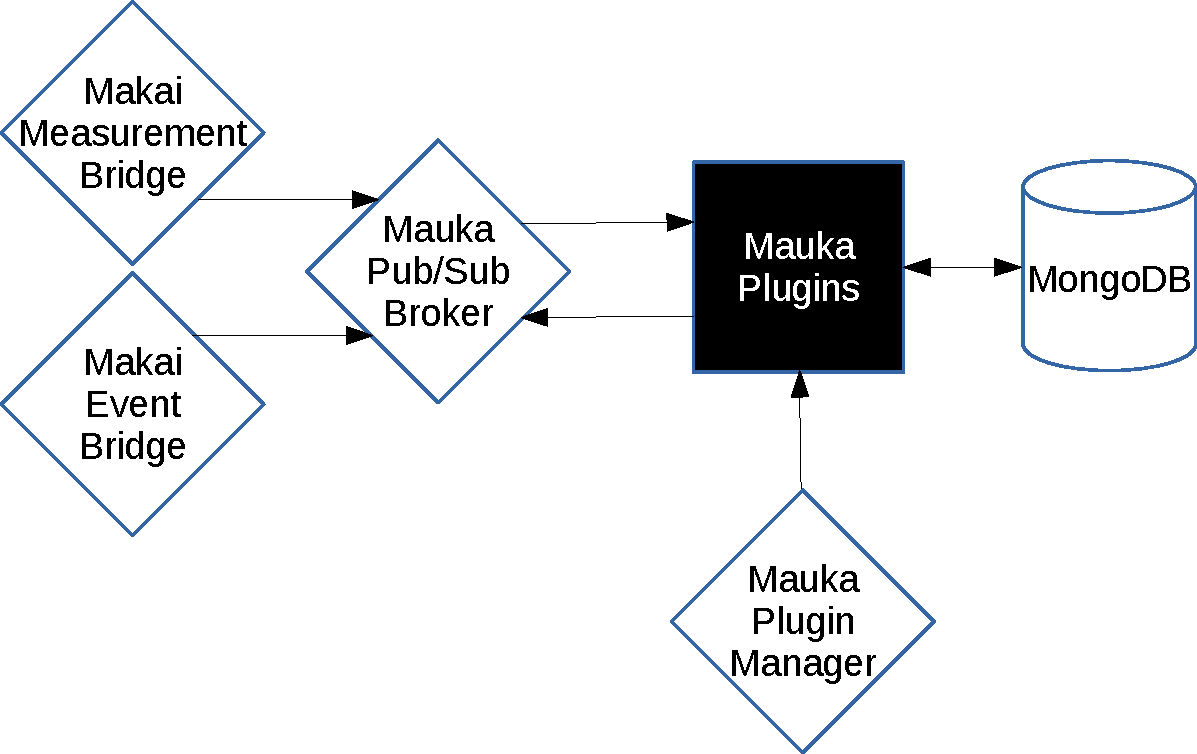
\includegraphics[width=0.6\textwidth]{img/mauka.pdf}
  \end{center}
  \caption{Block diagram of the OPQ Mauka.}
  \label{fig:8}
\end{figure}

Currently OPQMauka supports the following classification strategies: 
\begin{itemize}
	\item{\textbf{ITIC}} Power acceptability curve used to classify short term voltage sags.
	\item{\textbf{IEEE 1159 Voltage}} Voltage classification based on the IEEE 1159 power quality standard.
	\item{\textbf{Brownout Detection}} Classification of medium to long term voltage sags.
	\item{\textbf{Total Harmonic distortion}} Classification of events via harmonic analysis.
\end{itemize}

Once the anomaly is classified by OPQMauka, and the power quality characteristics are confirmed, it may be aggregated with other anomalies to form a disturbance. Disturbances are composed of raw box data, analysis results as well as expert annotations and other metadata.

\section{OPQView}

OPQView is the primary user interface to the OPQ echosystem. View is written in JavaScript using the meteor framework, and provides a robust and easy to use interface to the OPQBox triggering stream, Makai triggering anomalies, and to the Mauka PQ disturbances. Furthermore view provides an administration interface for initial setup and maintenance of the OPQ devices, and services. Finally OPQView monitors the health of the OPQ components, keeping track of the individual box uptimes, and component failures. A screenshot of the recent OPQ View build is shown in figure \ref{fig:9}

\begin{figure}[h]
  \begin{center}
  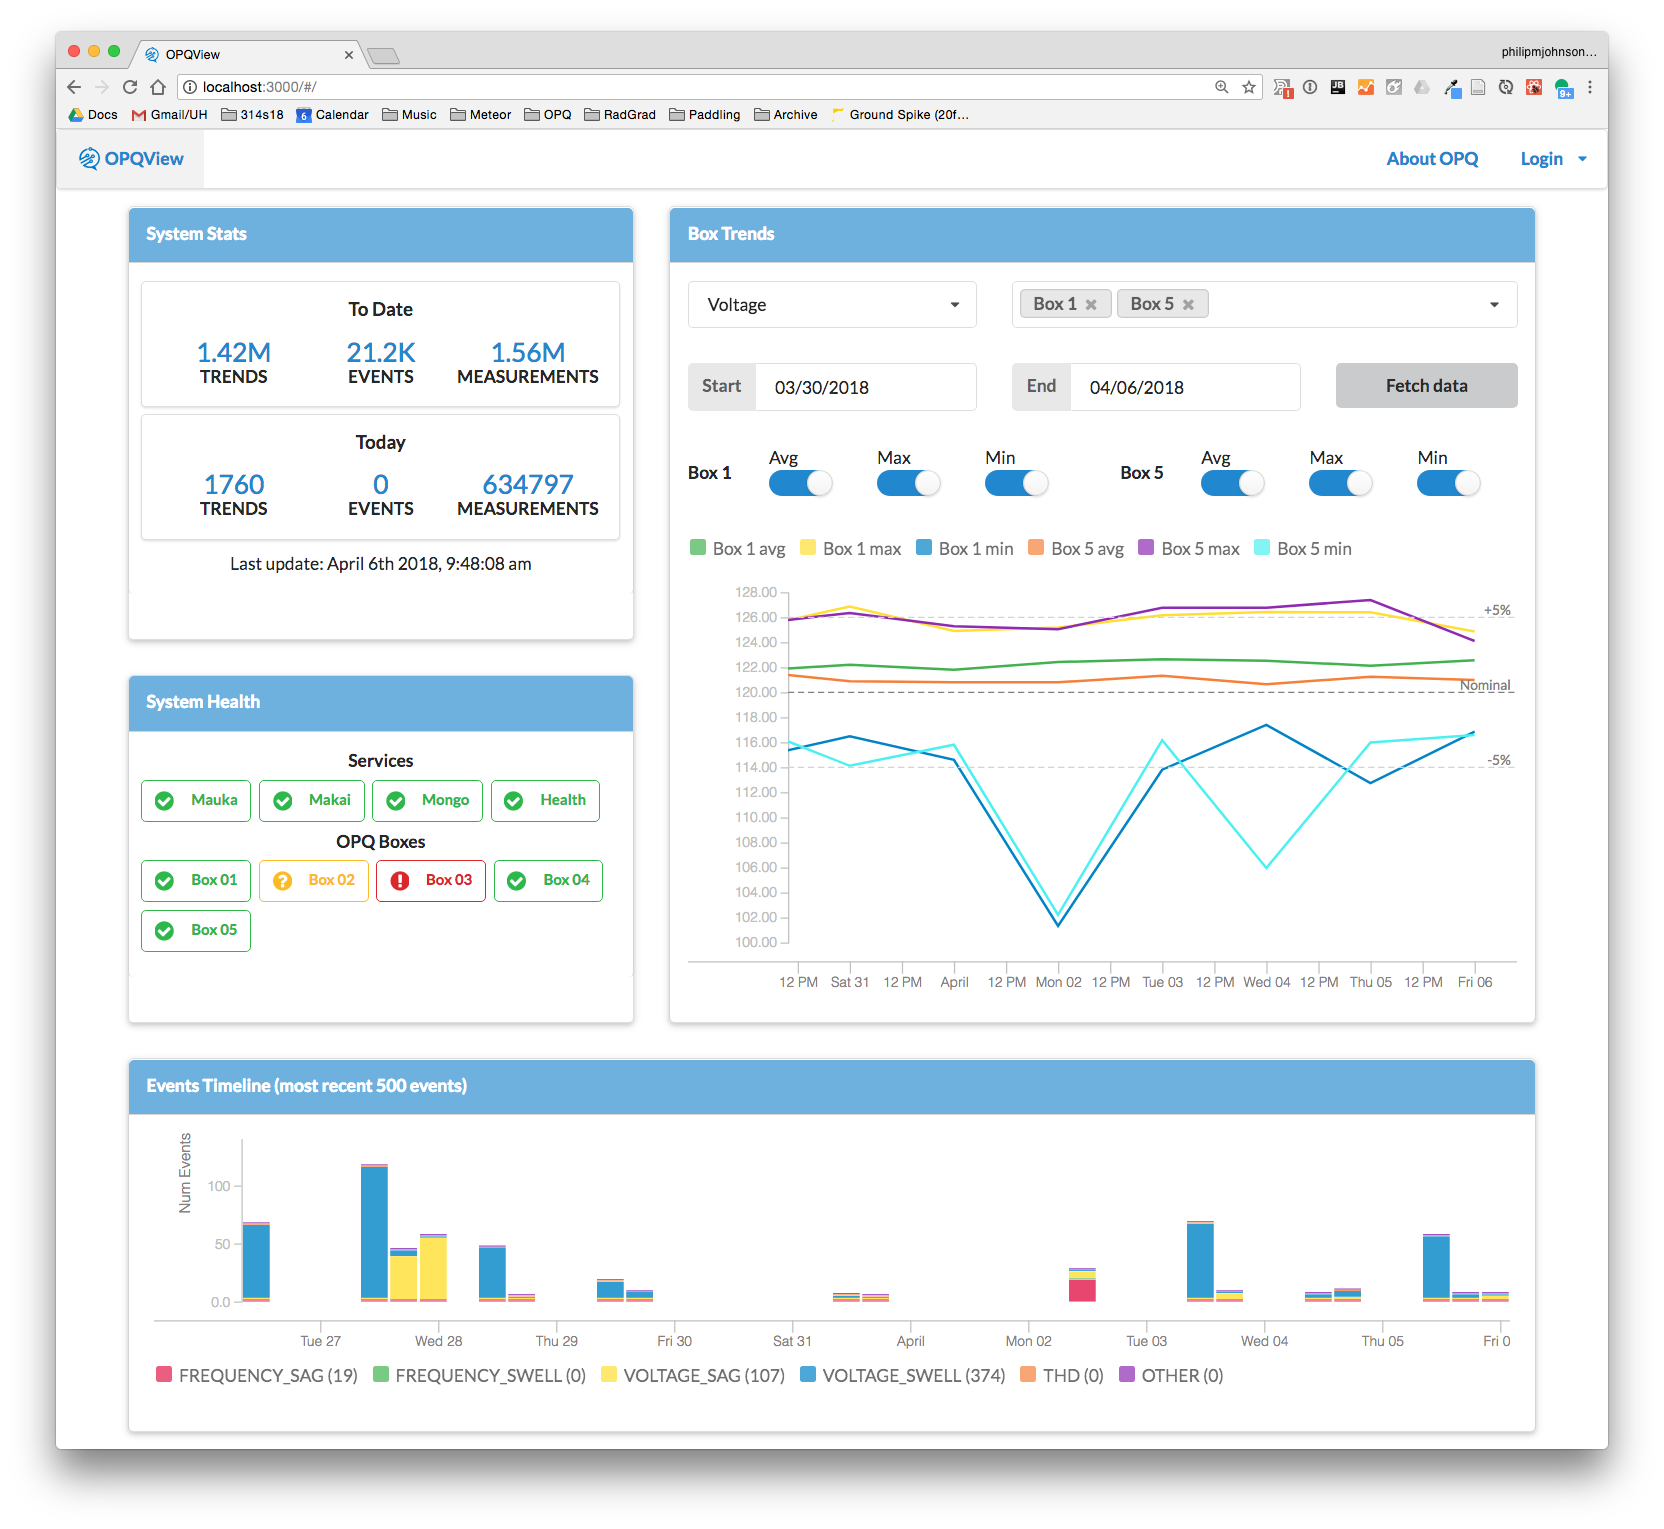
\includegraphics[width=0.6\textwidth]{img/opqview-landing-page.png}
  \end{center}
  \caption{Screenshot of a recent OPQView build.}
  \label{fig:9}
\end{figure}


\chapter{Experimental Design}
Validation of Napali hinges on the validation of performance of the OPQ Boxes. Some of the detection capability of the OPQ Boxes has already been characterized as shown in the previous section, however transient response and the $V_{rms}$ response are yet to be confirmed. Once the OPQ Box sensitivity has been characterized, the detection capability of Makai system must be crosschecked. First synthetic triggering streams will be injected into Makai. Next the full system will be deployed at the University of Hawaii Manoa for in-situ validation.

\section{OPQ Box Validation.}
So far only the frequency sensitivity of the OPQ Box has been validated empirically. The transient and as well as $V_{rms}$ response characterization will first be performed using synthetic data. Robust methods for generating power quality events are present in literature, and thus no new research for single device validation is required.\cite{kumar2015power}\cite{tan2013simulation} Next once the DSP software is characterized, synthetic PQ data will be loaded into a SDG1025 signal generator, and fed into the OPQ Box hardware. Any discrepancy between the DSP, and hardware-in-the-loop characterization will be noted and analyzed. The main characteristics to be validated are as follows:
\begin{itemize}
  \item{DC response:} Accuracy of the OPQ Box in measurement of a DC voltage.
  \item{$V_{rms}$ response:} Accuracy of the OPQ Box in measurement of a small changes in the amplitude of AC waveform.
  \item{THD response:} Accuracy of the OPQ Box in measurements of small harmonics mixed with a large fundamental AC waveform.
  \item{Transient response:} Validating the response of the OPQ Box metrics to various transients.
\end{itemize} 
These tests will provide a baseline for the detection capabilities of the Napali system, and result in a publication regarding the OPQ Box detection capabilities.

\section{Makai Synthetic Validation.}
While the synthetic data for a single point PQ disturbance is easily generated, distributed PQ event generation is not well developed. However there is some literature concerning power fault propagation and localization. \cite{parsons1998direction} \cite{polajvzer2017evaluation} The main takeaway from these authors is the energy and amplitude of the event diminishes with electrical distance from the source. As such, by generating a single point PQ event as described in \cite{kumar2015power}\cite{tan2013simulation}, and linearly scaling it based on the simulated electrical distance from the source, a distributed PQ event ensemble can be generated. These events will be ran through the simulated OPQ Box DSP stack and the metrics will be propagated to the Makai aggregation sink. Using these events as a baseline, I will be able to tune the threshold and temporal requirements for Makai detection algorithms. Furthermore, temporal, spacial, and amplitude noise will be injected into the generated datasets, to simulate various uncertainties with regards to data collection, such as local noise, and NTP errors. Finally single point PQ events will be injected into Makai to test the local event rejection capabilities.

\section{Napali in-situ Validation}
Once the OPQ Box is fully validated and the Makai detection thresholds are tuned using synthetic datasets, the Napali system will be fully deployed at the University of Hawaii at Manoa. In order to validate OPQ system as a whole it will be deployed across the University of Hawaii Manoa campus(UH). This location is ideal because it is a relatively isolated microgrid connected to the Oahu powergrid only via a single 46kV feeder as shown in figure \ref{expdes:fig:1}. Another advantage of the UH campus is the high number of smart meters deployed, across various levels of the power delivery infrastructure. While these meters are mainly geared towards monitoring power consumption they do have some power quality monitoring capabilities. Data provided from these meters can be used in two distinct applications. First of all, this data can be used to pinpoint the section of the University of Hawaii power grid which experience a higher likelihood of power quality disturbances. These portions of the grid will have a higher spacial density of OPQ Boxes. Secondly, data from the campus deployed meters can be used as ground truth for comparison against the measurements, and analysis performed by the OPQ project. The location of smart meters in the grid topology is shown in figure \ref{expdes:fig:1} as the $M$ nodes. As evident by the meter location none of them are monitoring the consumer level power and mainly focus on the higher voltage power delivery. This placement is evidenced from the smart meter role as a consumption monitor, and thus the deployment of the OPQ Boxes at the residential level will compliment the current power quality monitoring capabilities without introducing redundancies. Finally University of Hawaii powergrid is supplying a highly diverse infrastructure. Beyond the traditional residential equipment such as computers and consumer grade electronics, UH power grid powers scientific and laboratory equipment, machine shops, and server farms. All of these elements have varying requirements/tolerances for power quality anomalies as well as different levels of power quality "pollution". Furthermore some of the electricity consumers in the UH campus is entirely unique. For example the free electron laser located in the Watanabe Hall is one of the only free electron lasers in the world, and the impact/sensitivity of power quality on the instrument are completely unstudied.
\begin{figure}[h]
	\centering
	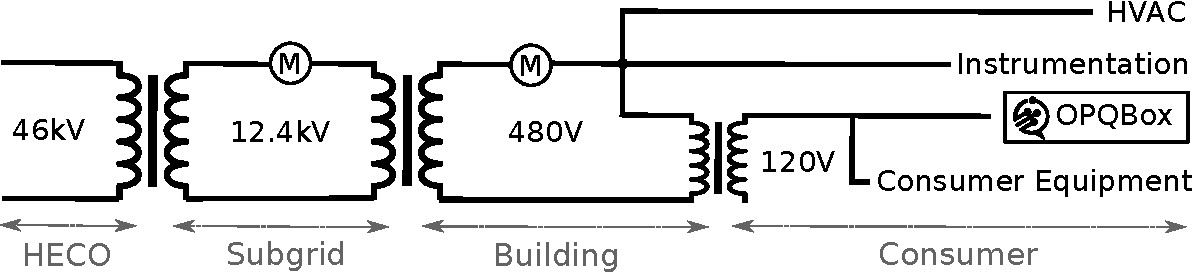
\includegraphics[width=1\linewidth]{img/uh-grid.pdf}	
	\caption{University of Hawaii at Manoa power delivery infrastructure.}
	\label{expdes:fig:1}
\end{figure}
Open power quality project acquired cloud infrastructure from the the Information Technology Services of University of Hawaii, which is hosted on the Manoa campus. This allows for low latency operation, and keeps all of the traffic constrained to the UH internal network. Furthermore UH hosts a Stratum 1 NTP server on its campus. This provides UH OPQ deployment with a low latency, high precision time keeping option. Finally, OPQ project received the Presidents Green Initiative Award in spring 2018. Besides a \$10,000 monetary award, this provides the OPQ project with access to all of the buildings on campus, expertise of the engineers who oversee the campus power infrastructure, as well as access to all of the smart meter measurements already deployed across campus. 

There are 74 smart meters deployed across the UH campus. These meters measure the fundamental frequency $V_{rms}$, power consumption, reactive power, and power factor. Data from these meters will be cross-referenced with the Napali detection system in order to ascertain it's benefits. Every time the Napali detects an event, both OPQ Boxes and building meters will be queried for data. While it may be unfeasible to query raw data from the UH metering infrastructure, metrics are readily available. This data will be used to ascertain the proportion of false positive events detected by Napali. Additional the internal single point fault detection mechanism of the UH power meters will be used in conjunction with the events detected by Napali to measure the rate of false negative events. Both the false negative and false positive measurements will be used to ascertain the detection efficient of the Napali framework. In order to analytically compute the bandwidth savings of the Napali compared to a system which sends all the data to the sink, I will keep track of the amount of bandwidth Napali monitoring system consumed during it`s deployment on UH campus. This will in turn be compared to the bandwidth required by the OPQ Boxes, if they were sending the entirety of the data to the sink, and establish the bandwidth efficiency of the Napali framework. The on-board cache for raw data will also be evaluated during the deployment. Taking into the account the detection latency of Makai, if some of the requested data is no longer available on the OPQ Box, only a partial time window will be returned. These events will be marked as incomplete and their fraction as compared to the total number of events recorded will be used to establish the latency tolerance of the Napali framework. Finally Napali methodology will be compared with the single point anomaly detection. In order to do that I will compare the extent to which the sub-threshold portion of events are missed by the UH metering infrastructure. In a large distributed event, if a portion of events is not detected by the UH meter`s single point detection, but picked up by the Napali framework, these events will be flagged and analyzed for their merit. This will in turn provide a metric of distributed detection ability of the Napali framework even without the raw data acquisition. Bellow is the time-line describing the major research activities leading up to my defense.


\begin{center}
\begin{tabular}{ ||c | c c|| }
\hline
 \textbf{Activity} & \textbf{Start Date} & \textbf{End Date} \\ 
 \hline
 \hline
 OPQ Box 2 Validation & October 1\textsuperscript{st} & November 31\textsuperscript{st} \\  
 Makai Validation & October 15 1\textsuperscript{st} & November 30\textsuperscript{th}   \\
 Data Collection & December 1\textsuperscript{st} & TBD   \\
 OPQ Box 2 Instrumentation paper & January 1\textsuperscript{st} & February 1\textsuperscript{st}   \\
 Data Analysis & February 1\textsuperscript{st} & March 1\textsuperscript{st}  \\
 Introduction Dissertation Chapter & March 1\textsuperscript{st}  & March 15\textsuperscript{th}  \\
 Literature Review Dissertation Chapter & March 15\textsuperscript{th} & April 1\textsuperscript{st}  \\
 Experimental Design Dissertation Chapter & April 1\textsuperscript{st} & April 15\textsuperscript{th}  \\
 Analysis Dissertation Chapter & April 15\textsuperscript{th} & May 15\textsuperscript{th}  \\
 Conclusions Dissertation Chapter & May 15\textsuperscript{th} & June 15\textsuperscript{th}  \\
 \hline
 
\end{tabular}
\end{center}


\chapter{Conclusions}


\bibliography{proposal.bib} 
\bibliographystyle{plain}
  
\end{document}
